% !TEX program = xelatex
\documentclass[a4paper,11pt]{ctexart}

\usepackage[margin=2.4cm,headheight=14pt]{geometry}
\usepackage{xeCJK}
\setCJKmainfont[BoldFont=Songti SC Bold]{Songti SC}
\setCJKsansfont[BoldFont=STHeiti]{STHeiti}
\setCJKmonofont{STHeiti}
\setmainfont{Times New Roman}
\setmonofont[Scale=0.82]{Menlo}

\usepackage{graphicx}
\usepackage{longtable}
\usepackage{tabularx}
\usepackage{array}
\usepackage{booktabs}
% \usepackage{ltablex}\keepXColumns  % not available; use longtable + tabularx separately
\usepackage{xcolor}
\usepackage{fancyhdr}
\usepackage[colorlinks=true,linkcolor=blue!60!black,urlcolor=blue!60!black]{hyperref}

\graphicspath{{diagrams/}}

\definecolor{accent}{HTML}{1F4E79}
\definecolor{rowstripe}{HTML}{F4F8FC}

% titlesec unavailable; use ctex defaults but color section heads via redefinition
\ctexset{
  section/format = \Large\bfseries\color{accent},
  subsection/format = \large\bfseries\color{accent!90!black},
  subsubsection/format = \normalsize\bfseries
}

\setlength{\parindent}{2em}
\setlength{\parskip}{0.35em}
\renewcommand{\arraystretch}{1.2}

\newcolumntype{Y}{>{\raggedright\arraybackslash}X}
\newcolumntype{L}[1]{>{\raggedright\arraybackslash}p{#1}}

\pagestyle{fancy}
\fancyhf{}
\rhead{\small 智能充电桩调度计费系统 · HW2}
\lhead{\small 第\ \thepage\ 页}
\renewcommand{\headrulewidth}{0.3pt}

\title{\vspace{-1.2cm}\textbf{智能充电桩调度计费系统}\\[6pt]\large 动态结构与静态结构设计}
\author{组长：唐振桓 \quad 组员：杨凌俊、袁炜途、马迪轩、刘宇轩}
\date{2026 年 6 月 2 日}

\begin{document}
\maketitle
\thispagestyle{empty}


\tableofcontents
\newpage

%==========================================================
\section{系统架构选择及说明 (10\%)}

\subsection{架构选型}

需求说明书有三个核心约束：(1) 系统由``服务器端 + 用户客户端 + 管理员客户端''三方构成；(2) 排队调度、计费、故障恢复都需要全局一致的状态；(3) 充电桩状态需要在客户端定时刷新。综合这三点，我们采用``\textbf{C/S 架构 + 三层逻辑分层 + 服务端 MVC}''的方案，并在服务器内部按 Boundary–Control–Entity（BCE）划分协作对象，方便在第二章的时序图里把每个事件画清楚。

之所以没有选 B/S：管理员要长轮询桩的状态，用户要接收``叫号''推送，而系统部署在校内私网，C/S 在长连接、即时通知和本地缓存上比一般 B/S 更顺手。也没有选微服务：5 个桩 + 1 个充电站的规模根本不需要拆服务，反倒会让调度一致性更难维护。

\subsection{物理部署与运行视图}

\begin{figure}[ht]
\centering
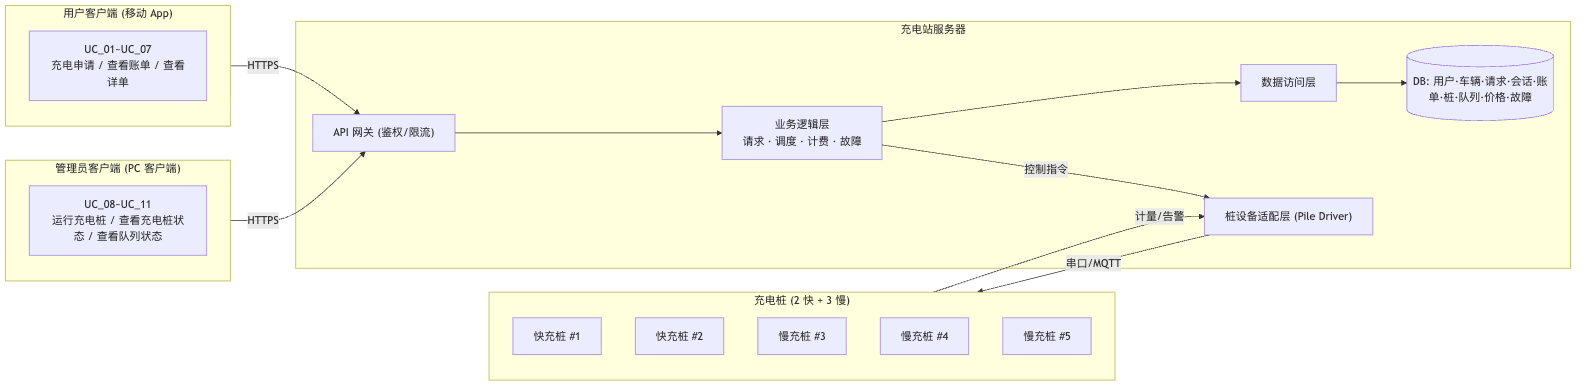
\includegraphics[width=0.95\linewidth]{diagram_01.png}
\caption{物理部署与运行视图}
\end{figure}

充电桩本身不直接对客户端开放：所有控制指令（启动、停止、参数下发）和状态回采（计量、告警）都过服务器的``桩设备适配层''。这样状态在服务端有唯一可信副本，调度才好做。

\subsection{三层逻辑分层}

\begin{longtable}{p{3.6cm}p{6cm}p{6cm}}
\toprule
\textbf{层} & \textbf{主要职责} & \textbf{对应类型示例} \\
\midrule
\endhead
表示层 (Presentation) & 屏幕渲染、表单校验、推送接收、本地缓存 & \texttt{UserClient} / \texttt{AdminClient} 及其内部 View/ViewModel \\
业务逻辑层 (Business Logic) & 用例级控制逻辑、调度算法、计费规则、超时与故障策略 & \texttt{ChargeRequestController} / \texttt{ScheduleManager} / \texttt{BillingService} / \texttt{FaultService} / \texttt{PileService} \\
数据访问层 (Data Access) & 持久化、事务、唯一性约束、并发控制 & \texttt{RequestRepo} / \texttt{SessionRepo} / \texttt{BillRepo} / \texttt{PileRepo} / \texttt{PriceRepo} \\
\bottomrule
\end{longtable}

\subsection{服务器内部职责划分}

服务器在业务逻辑层内部采用 BCE 模式：

\begin{itemize}
\item \textbf{Boundary（边界对象）}：每个用例对应一个 \texttt{XxxController}，做鉴权、参数校验，把客户端协议消息映射成内部消息。
\item \textbf{Control（控制对象）}：跨多个实体协调的服务对象，例如 \texttt{ScheduleManager}（排队/分桩）、\texttt{BillingService}（计费）、\texttt{FaultService}（故障）。
\item \textbf{Entity（实体对象）}：HW1 领域模型 18 个类的实现，承担属性持久化和不变量自检。
\end{itemize}

第二章每张时序图里的 lifeline 都按这个划分，对象命名用 \texttt{:ClassName}，箭头采用 UML 2 标准。

\subsection{与本次作业的对应关系}

\begin{itemize}
\item 本章（10\%）给出整体架构图和分层，做为后两章的上下文。
\item 第二章（80\%）的所有系统事件都落在``客户端 → API 网关 → Controller → Service → Entity → Repo''这条链路上；调度和故障部分会额外用到 \texttt{ScheduleManager} 与 \texttt{FaultService} 之间的内部交互。
\item 第三章（10\%）只保留与系统事件直接相关的类，按作业要求仅使用依赖、定向关联、继承三种关系。
\end{itemize}

\clearpage
%==========================================================
\section{动态结构设计 (80\%)}

\subsection{设计概览与统一图例}

本章共给出 \textbf{15} 个必做系统事件的时序图、\textbf{3} 个组长完成的调度对象交互图，以及 \textbf{2} 个可选加分调度策略的时序图，合计 \textbf{20} 张 UML Sequence Diagram。每个用例按模版组织：``已知条件 $\to$ 对象设计（操作契约 + 问题/解决方案 + sequence diagram）''，一直写到该用例最后一条消息。

为了让各张图风格一致，时序图遵循以下约定：

\begin{enumerate}
\item 全部使用 UML 2 sequence diagram 记法；同步消息用实心三角箭头，异步消息用细线开放箭头，返回值用虚线箭头。
\item lifeline 命名为 ``角色 / :类名''，同一个类在不同图里保持同名。
\item 控制结构使用 \texttt{alt / opt / loop / par} 复合片段，约束写在 \texttt{note} 中。
\item 系统事件名（来自作业要求表）在第一条消息上以加粗形式显示，参数列表与原表完全一致。
\item 与 HW1 操作契约保持一致：前置条件不满足走 \texttt{alt 异常} 分支返回错误码 \texttt{1}；正常路径返回 \texttt{0} 或题目要求的对象。
\end{enumerate}

下表列出全章会反复出现的核心对象：

\begin{longtable}{p{2.4cm}p{4.4cm}p{2.2cm}p{6cm}}
\toprule
\textbf{简写} & \textbf{全名} & \textbf{所在层} & \textbf{角色} \\
\midrule
\endhead
\texttt{:UserClient} & 用户客户端 & 表示层 & 用户操作入口 \\
\texttt{:AdminClient} & 管理员客户端 & 表示层 & 管理员操作入口 \\
\texttt{:ChargeReqCtrl} & \texttt{:ChargeRequestController} & 业务边界 & 充电申请系列用例的 Controller \\
\texttt{:BillCtrl} & \texttt{:BillController} & 业务边界 & 账单/详单用例的 Controller \\
\texttt{:PileCtrl} & \texttt{:PileController} & 业务边界 & 运行/查询充电桩用例的 Controller \\
\texttt{:QueueCtrl} & \texttt{:QueueController} & 业务边界 & 查看队列状态用例的 Controller \\
\texttt{:ScheduleMgr} & \texttt{:ScheduleManager} & 业务控制 & 调度算法与队列调度入口 \\
\texttt{:BillingSvc} & \texttt{:BillingService} & 业务控制 & 计费、生成账单与详单 \\
\texttt{:FaultSvc} & \texttt{:FaultService} & 业务控制 & 故障识别、再调度、故障恢复 \\
\texttt{:PileSvc} & \texttt{:PileService} & 业务控制 & 充电桩生命周期（上电/启动/关闭） \\
\texttt{:WaitingArea} & 等候区 & 实体 & 持有两个等待队列 \\
\texttt{:WaitingQueue} & 等待队列（快/慢） & 实体 & FIFO 队列 \\
\texttt{:ChargingArea} & 充电区 & 实体 & 持有 5 个充电桩 \\
\texttt{:ChargingPile} & 充电桩 & 实体 & 桩内 4 位排队队列 \\
\texttt{:Req} & \texttt{:ChargingRequest} & 实体 & 单次请求生命周期对象 \\
\texttt{:Session} & \texttt{:ChargingSession} & 实体 & 充电会话（实时电量、时长） \\
\texttt{:Bill} & \texttt{:Bill} & 实体 & 一次会话对应一份账单/详单 \\
\texttt{:PricingRule} & 分时电价规则 & 实体 & 三段式电价 \\
\texttt{:ServiceRule} & 服务费规则 & 实体 & 服务费率 \\
\texttt{:PileDriver} & 桩设备适配层 & 设备 & 与物理桩交换控制/计量信号 \\
\texttt{:RequestRepo} & 请求 DAO & 数据访问 & 充电请求的持久化与查询 \\
\texttt{:SessionRepo} & 会话 DAO & 数据访问 & 充电会话的持久化与查询 \\
\texttt{:BillRepo} & 账单 DAO & 数据访问 & 账单的查询与落盘 \\
\texttt{:PileRepo} & 桩 DAO & 数据访问 & 桩状态与累计计数器 \\
\texttt{:PriceRepo} & 电价 DAO & 数据访问 & 电价规则、服务费规则的版本化存储 \\
\bottomrule
\end{longtable}

作业要求表中的英文消息名（例如 \texttt{E\_chargingRequest}）属于``系统事件''层面，对应 HW1 操作契约里的 \texttt{SubmitChargeRequest} 等编程名。本章在每张图的第一条消息上严格使用作业要求表里的命名，以满足``标黄系统事件''的覆盖要求。

\clearpage
%==========================================================
\subsection{用例：充电申请}

\subsubsection{已知条件}

本用例下所有系统事件及对应返回值如下表（与作业要求表完全一致），每条系统事件对应的操作契约在下文``对象设计''小节里作为已知条件分别给出。

\begin{longtable}{cp{2.4cm}p{6.2cm}p{5.6cm}}
\toprule
\textbf{序号} & \textbf{指令} & \textbf{系统事件} & \textbf{返回} \\
\midrule
\endhead
1 & 提交充电申请 & \texttt{E\_chargingRequest(car\_Id, Request\_Amount, Request\_Mode)} & \texttt{Return(car\_position, car\_state, queue\_Num, request\_time)} \\
2 & 修改充电量 & \texttt{Modify\_Amount(car\_Id, Amount)} & \texttt{Return(0/1)} \\
3 & 修改充电模式 & \texttt{Modify\_Mode(car\_Id, Mode)} & \texttt{Return(0/1)} \\
4 & 查看队列状态 & \texttt{Query\_Car\_State(car\_Id)} & \texttt{Return(car\_Number\_before\_position, car\_state, queue\_Num, request\_time)} \\
5 & 开始充电 & \texttt{Start\_Charging(car\_Id, ChargePileNum)} & \texttt{Return(0/1)} \\
6 & 查看充电状态 & \texttt{Query\_Charging\_State(car\_Id)} & \texttt{Return(详单信息)} \\
7 & 结束充电 & \texttt{End\_Charging(car\_Id, ChargePileNum)} & \texttt{Return(0/1)} \\
\bottomrule
\end{longtable}

\subsubsection{对象设计：E\_chargingRequest(car\_Id, Request\_Amount, Request\_Mode)}

\textbf{(1) 操作契约（已知条件）}

\begin{longtable}{p{2.4cm}p{13cm}}
\toprule
\textbf{项目} & \textbf{内容} \\
\midrule
\endhead
系统事件 & \texttt{E\_chargingRequest(car\_Id, Request\_Amount, Request\_Mode)} \\
交叉引用 & UC\_01 充电申请 — 提交充电申请 \\
前置条件 & 1. 车辆 \texttt{car\_Id} 已通过等候区入场鉴权。 2. 用户和车辆身份有效。 3. 当前不存在该车辆未完成的有效充电请求。 4. 用户不存在未支付且已超期的账单限制。 \\
后置条件 & 1. 创建一个新的 \texttt{:ChargingRequest}。 2. 与 \texttt{:User}、\texttt{:Vehicle} 建立关联。 3. 根据 \texttt{Request\_Mode} 加入对应模式的 \texttt{:WaitingQueue}。 4. 初始化请求 \texttt{state=排队中}、记录 \texttt{request\_time}、\texttt{target\_amount=Request\_Amount}，由队列分配 \texttt{queue\_Num}。 5. 更新等待队列长度与预计等待时长。 6. 向客户端返回 \texttt{car\_position / car\_state / queue\_Num / request\_time}。 \\
\bottomrule
\end{longtable}

\noindent\textbf{(2) 问题与解决方案}

\begin{tabularx}{\linewidth}{p{5cm}Y}
\toprule
\textbf{问题} & \textbf{解决方案} \\
\midrule
第一个接收该消息的软件对象是谁？ & 后台边界对象 \texttt{:ChargeRequestController}，负责鉴权、参数校验，并把外部消息转为内部领域消息。 \\
谁负责创建 \texttt{:ChargingRequest} 实例？ & \texttt{:ScheduleManager} 在 \texttt{createRequest()} 中创建实例，并委托 \texttt{:RequestRepo} 持久化。 \\
哪些对象之间需要建立关联？ & 新建 \texttt{:ChargingRequest} 通过 \texttt{:WaitingArea.getQueue(mode)} 找到对应 \texttt{:WaitingQueue}，再 \texttt{enqueue} 进去；同时记录 \texttt{User/Vehicle} 引用。 \\
哪些属性需要初始化或修改？ & \texttt{:ChargingRequest} 的 \texttt{state=排队中}、\texttt{request\_time=now}、\texttt{target\_amount=Request\_Amount}、\texttt{queue\_Num} 由 \texttt{:WaitingQueue} 分配；\texttt{:WaitingQueue.size++}。 \\
是否需要数据持久化对象？ & 是。\texttt{:RequestRepo} 通过 \texttt{save(:Req)} 把新请求落到 \texttt{requests} 表。 \\
\bottomrule
\end{tabularx}

\textbf{(3) Sequence Diagram}

\begin{figure}[ht]
\centering
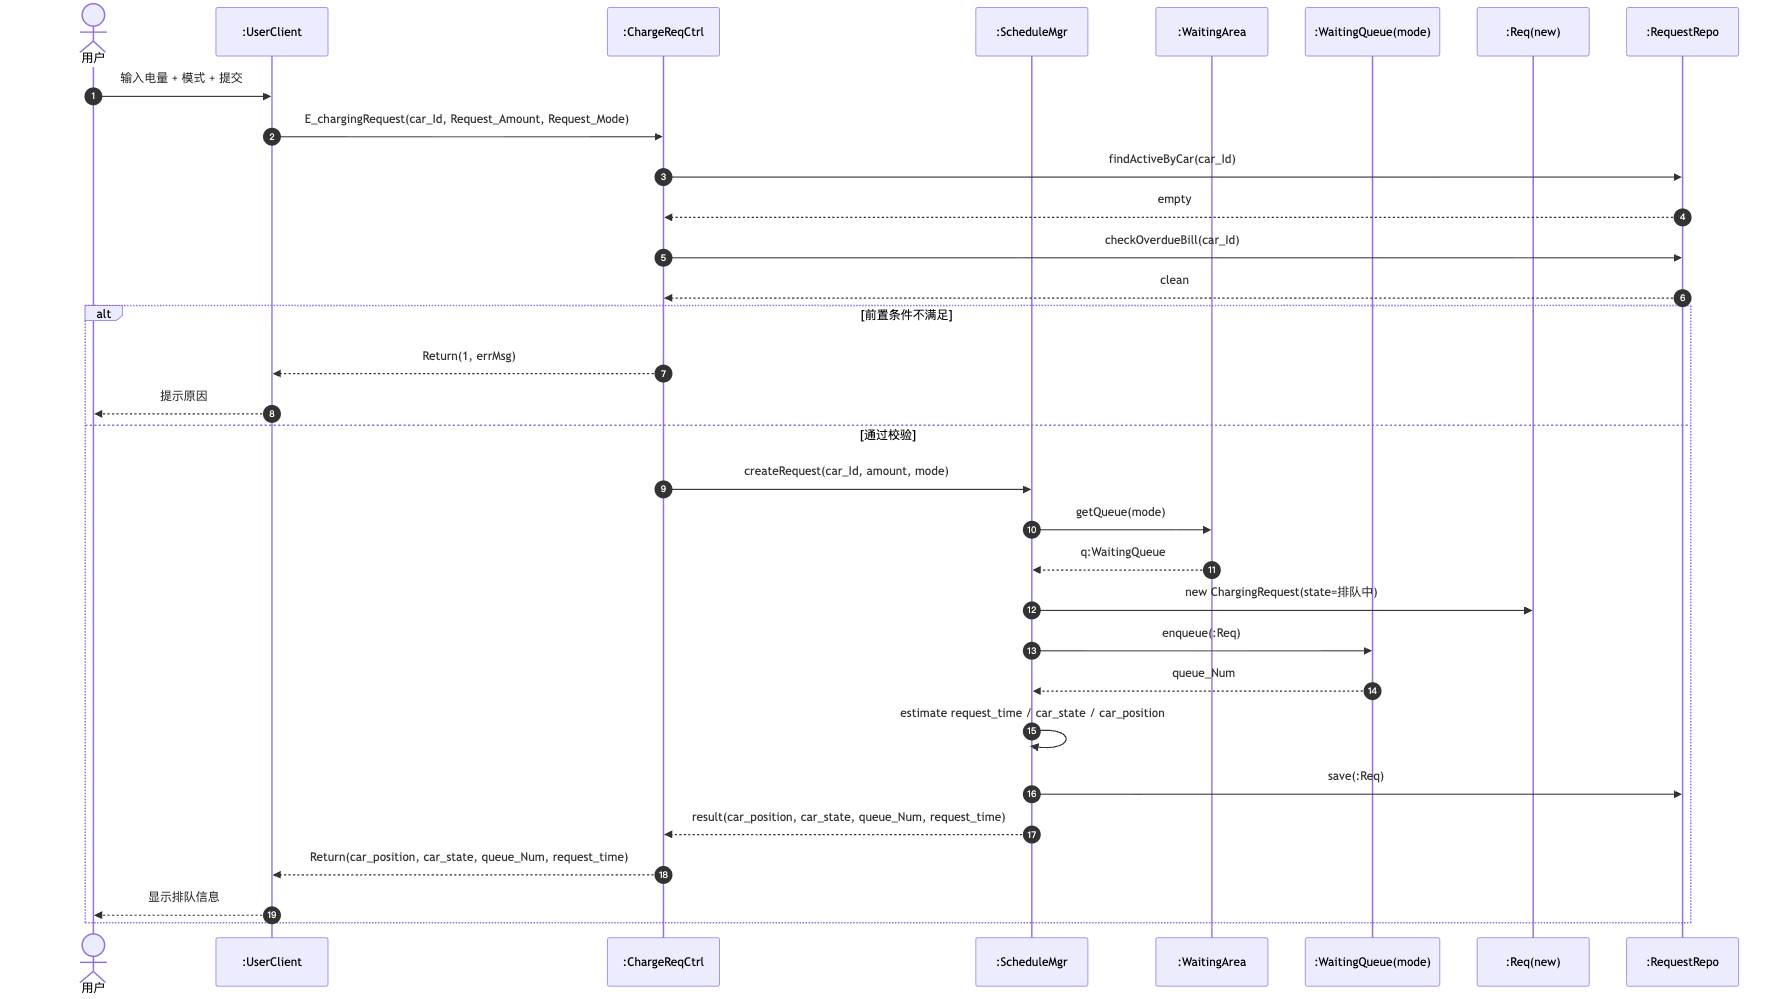
\includegraphics[width=0.95\linewidth]{diagram_02.png}
\end{figure}

\noindent 说明：\texttt{car\_state} 取值与 HW1 一致，包含``排队中 / 已调度未开始 / 充电中 / 已完成 / 已取消''。

\subsubsection{对象设计：Modify\_Amount(car\_Id, Amount)}

\textbf{(1) 操作契约（已知条件）}

\begin{tabularx}{\linewidth}{p{2.4cm}Y}
\toprule
\textbf{项目} & \textbf{内容} \\
\midrule
系统事件 & \texttt{Modify\_Amount(car\_Id, Amount)} \\
交叉引用 & UC\_01 充电申请 — 修改充电量 \\
前置条件 & 1. 对应 \texttt{:ChargingRequest} 存在。 2. 请求当前状态为``排队中''或``已调度未开始充电''。 3. 新的目标电量 \texttt{Amount > 0} 且符合业务规则。 \\
后置条件 & 1. 原 \texttt{:ChargingRequest.target\_amount} 被更新为 \texttt{Amount}。 2. 由 \texttt{:ScheduleManager} 重新估算等待时长。 3. 仅修改电量，不重排队、不生成新请求。 4. 返回 \texttt{0}（成功）或 \texttt{1}（拒绝）。 \\
\bottomrule
\end{tabularx}

\noindent\textbf{(2) 问题与解决方案}

\begin{tabularx}{\linewidth}{p{5cm}Y}
\toprule
\textbf{问题} & \textbf{解决方案} \\
\midrule
谁负责接收该消息？ & \texttt{:ChargeRequestController} 继续作为充电申请系列用例的边界。 \\
谁负责状态校验？ & 控制器查 \texttt{:RequestRepo} 获得当前请求，再读 \texttt{:Req.state}；若已进入 \texttt{充电中} 直接返回 \texttt{1}。 \\
哪些对象需要交互？ & \texttt{:ChargeReqCtrl} 调用 \texttt{:Req.setTargetAmount(Amount)} 和 \texttt{:ScheduleMgr.recomputeWaitTime(:Req)}。 \\
哪些属性发生修改？ & \texttt{:Req.target\_amount} 改为 \texttt{Amount}，\texttt{:Req.modified\_at = now}。 \\
\bottomrule
\end{tabularx}

\textbf{(3) Sequence Diagram}

\begin{figure}[ht]
\centering
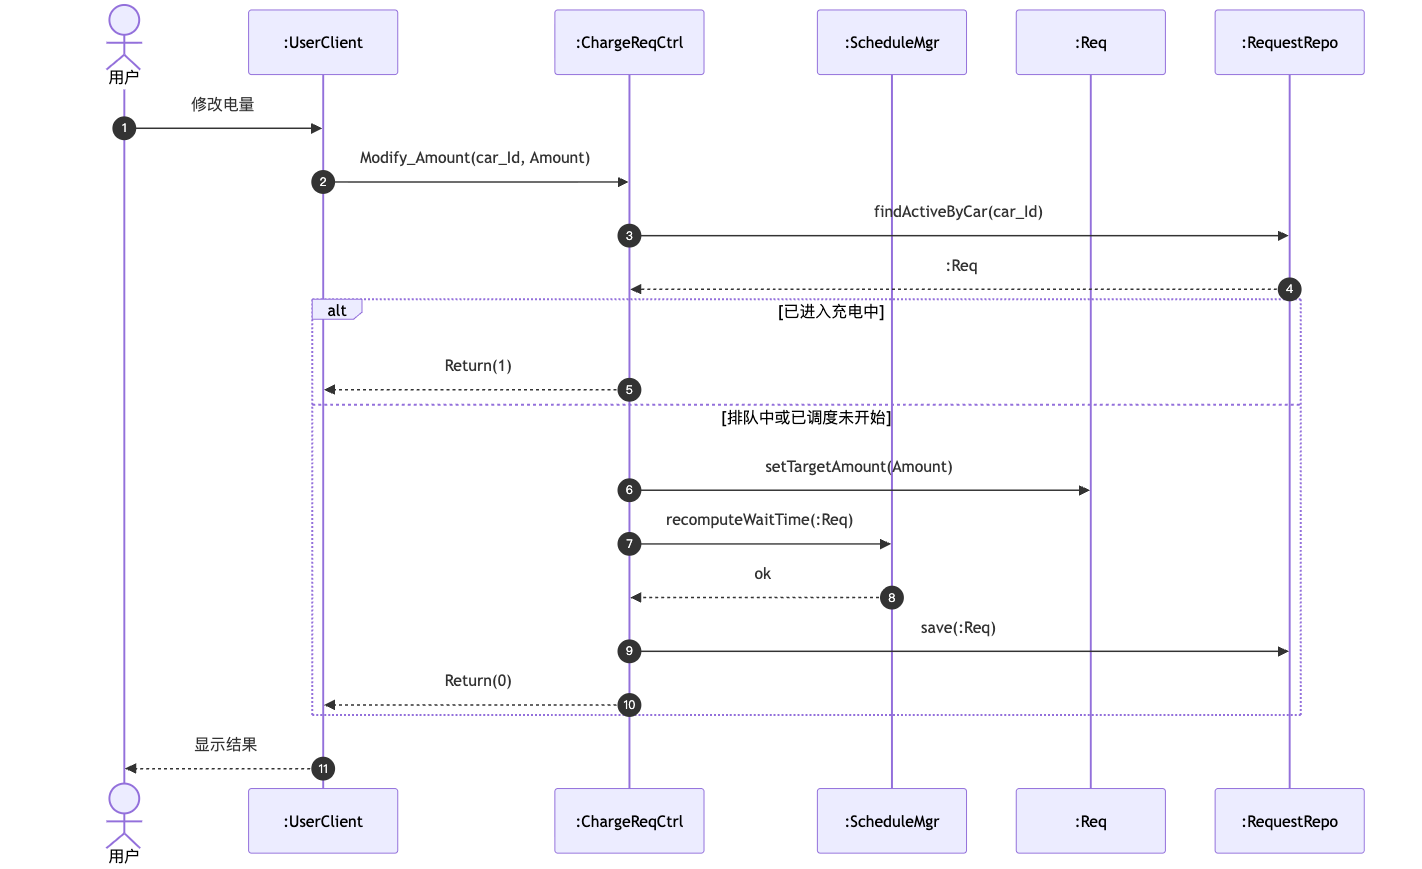
\includegraphics[width=0.85\linewidth]{diagram_03.png}
\end{figure}

\subsubsection{对象设计：Modify\_Mode(car\_Id, Mode)}

\textbf{(1) 操作契约（已知条件）}

\begin{tabularx}{\linewidth}{p{2.4cm}Y}
\toprule
\textbf{项目} & \textbf{内容} \\
\midrule
系统事件 & \texttt{Modify\_Mode(car\_Id, Mode)} \\
交叉引用 & UC\_01 充电申请 — 修改充电模式 \\
前置条件 & 1. 对应 \texttt{:ChargingRequest} 存在。 2. 请求状态为``排队中''或``已调度未开始充电''。 3. \texttt{Mode} 与当前模式不同。 \\
后置条件 & 1. 原 \texttt{:ChargingRequest} 标记为``已取消''并从原 \texttt{:WaitingQueue} 移除。 2. 新建一个 \texttt{:ChargingRequest}，模式为 \texttt{Mode}，按公平原则插到新模式队列尾部。 3. 重新估算等待时长。 4. 返回新的 \texttt{queue\_Num}。 \\
\bottomrule
\end{tabularx}

\noindent\textbf{(2) 问题与解决方案}

\begin{tabularx}{\linewidth}{p{5cm}Y}
\toprule
\textbf{问题} & \textbf{解决方案} \\
\midrule
为何不能在原 \texttt{:Req} 上原地切换模式？ & 业务规则要求``换队即重排''来避免插队，所以必须取消旧请求并以新模式重新排队。 \\
谁负责创建新请求？ & \texttt{:ChargeRequestController} 直接 \texttt{new ChargingRequest(mode=Mode)}，并委托 \texttt{:ScheduleMgr} 估算新等待时长。 \\
哪些 \texttt{:WaitingQueue} 受影响？ & 旧模式队列执行 \texttt{remove(:Req(old))}；新模式队列执行 \texttt{enqueue(:Req(new))}。 \\
哪些属性需要修改？ & \texttt{:Req(old).state=已取消}、\texttt{:Req(new).state=排队中}、\texttt{:Req(new).queue\_Num} 由新队列分配。 \\
\bottomrule
\end{tabularx}

\textbf{(3) Sequence Diagram}

\begin{figure}[ht]
\centering
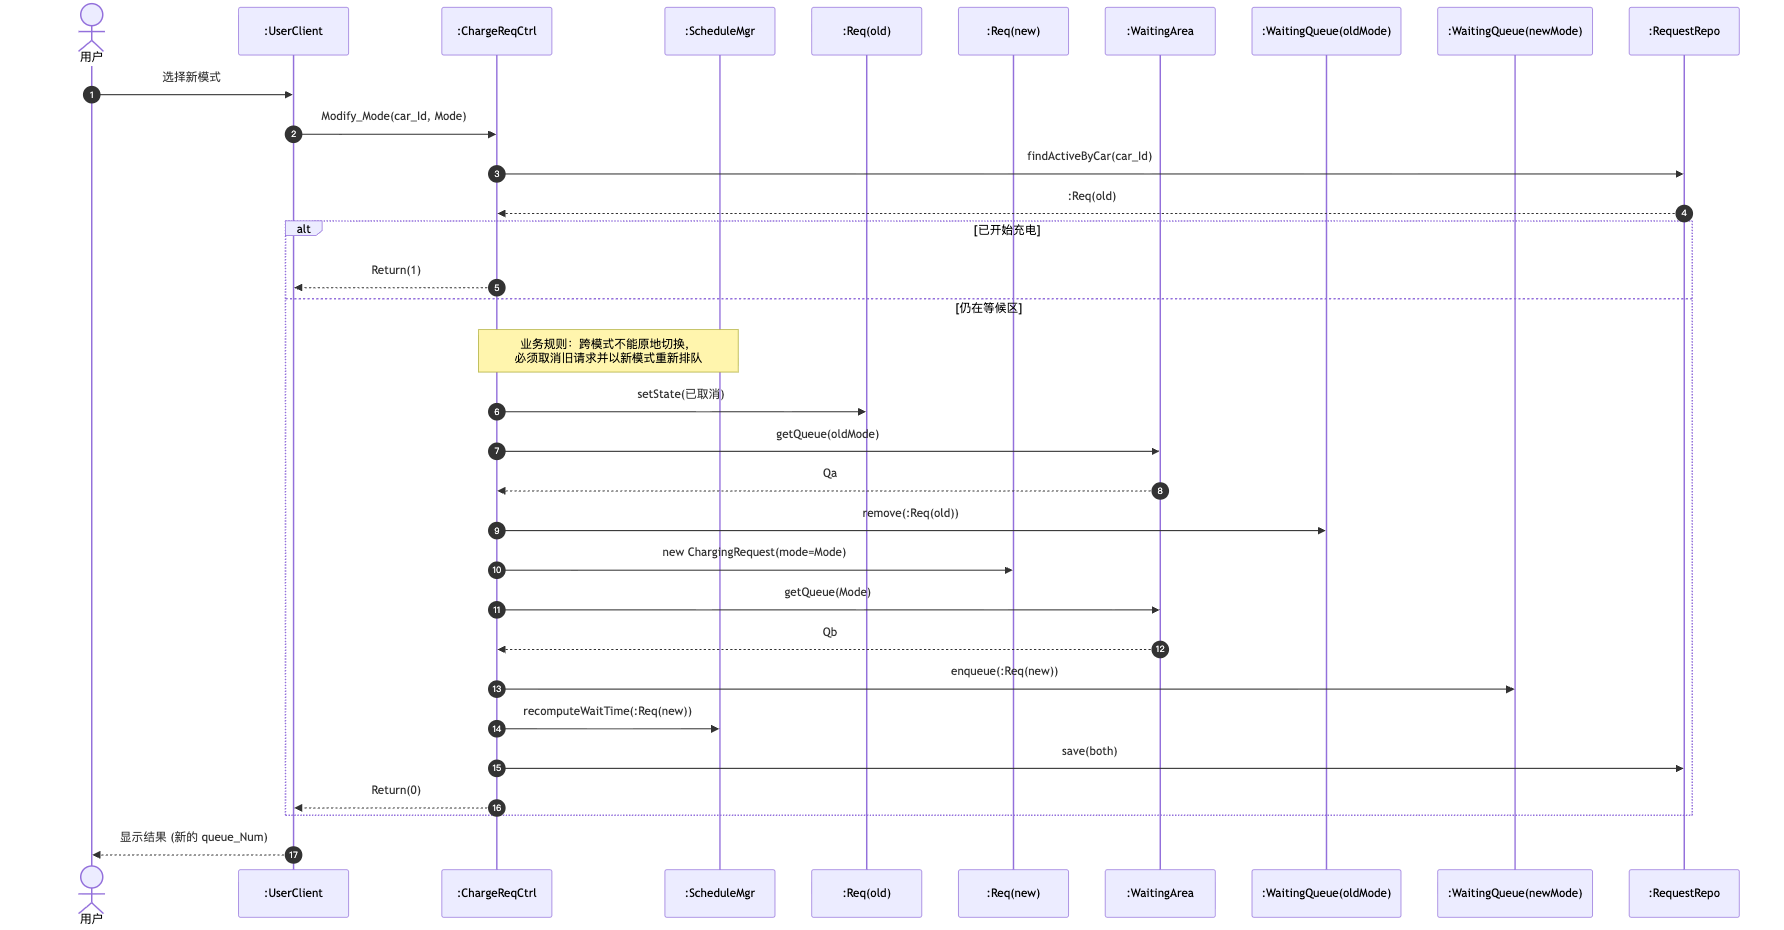
\includegraphics[width=0.95\linewidth]{diagram_04.png}
\end{figure}

\subsubsection{对象设计：Query\_Car\_State(car\_Id)}

\textbf{(1) 操作契约（已知条件）}

\begin{tabularx}{\linewidth}{p{2.4cm}Y}
\toprule
\textbf{项目} & \textbf{内容} \\
\midrule
系统事件 & \texttt{Query\_Car\_State(car\_Id)} \\
交叉引用 & UC\_01 充电申请 — 查看队列状态 \\
前置条件 & 1. 对应 \texttt{:ChargingRequest} 存在且状态非终态（不是``已完成''/``已取消''）。 2. 用户具备查询该请求的权限。 \\
后置条件 & 1. 读取该 \texttt{:Req} 当前 \texttt{state}、所属 \texttt{:WaitingQueue}、排队位置和预计等待时间。 2. 不修改任何持久化业务对象，只返回最新队列视图。 \\
\bottomrule
\end{tabularx}

\noindent\textbf{(2) 问题与解决方案}

\begin{tabularx}{\linewidth}{p{5cm}Y}
\toprule
\textbf{问题} & \textbf{解决方案} \\
\midrule
谁负责拼装返回视图？ & \texttt{:ChargeRequestController} 编排查询，组合 \texttt{:Req} 自身属性与 \texttt{:WaitingQueue.positionOf()} 的结果。 \\
为何不直接读 \texttt{:WaitingQueue.list()}？ & 队列长度可能远大于该请求所需信息，只取 \texttt{positionOf} 可以省传输与计算量。 \\
是否会触发副作用？ & 无。\texttt{Query} 是只读视图，必须保证不修改任何业务对象状态。 \\
\bottomrule
\end{tabularx}

\textbf{(3) Sequence Diagram}

\begin{figure}[ht]
\centering
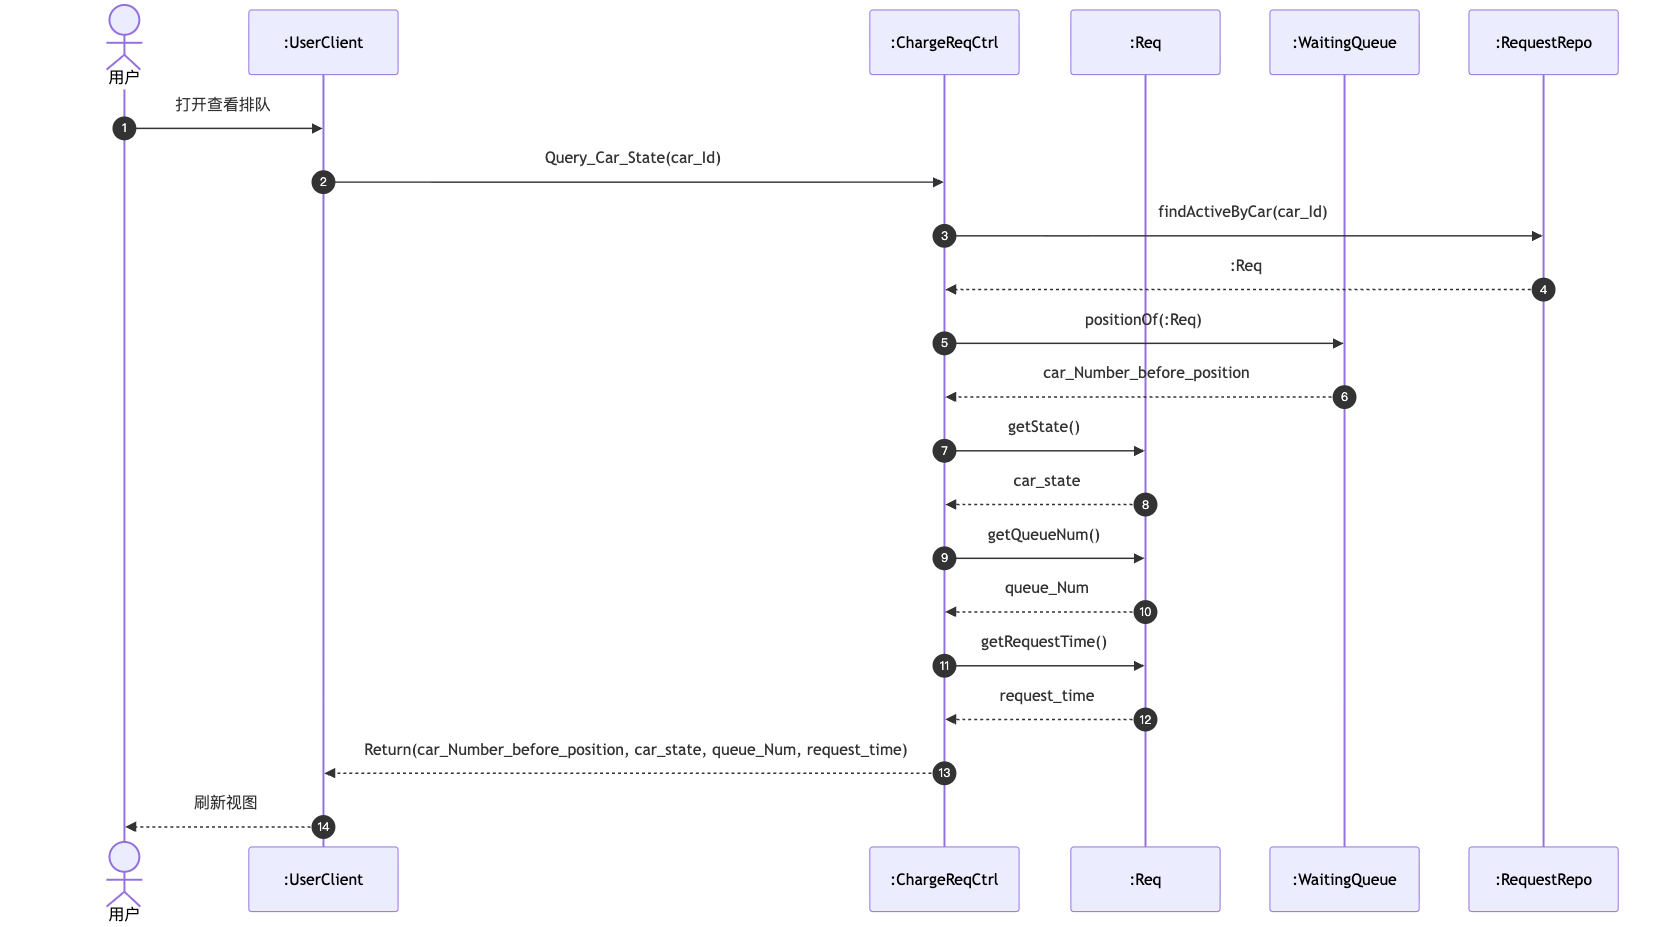
\includegraphics[width=0.85\linewidth]{diagram_05.png}
\end{figure}

\subsubsection{对象设计：Start\_Charging(car\_Id, ChargePileNum)}

\textbf{(1) 操作契约（已知条件）}

\begin{tabularx}{\linewidth}{p{2.4cm}Y}
\toprule
\textbf{项目} & \textbf{内容} \\
\midrule
系统事件 & \texttt{Start\_Charging(car\_Id, ChargePileNum)} \\
交叉引用 & UC\_01 充电申请 — 开始充电 \\
前置条件 & 1. 该 \texttt{:Req} 已被调度到 \texttt{ChargePileNum} 对应的 \texttt{:ChargingPile}。 2. 用户在 5 分钟叫号窗口内确认入场。 3. 该桩当前处于``空闲''或``占用但已就绪''状态。 4. 该车在桩内排队队首。 \\
后置条件 & 1. 创建新的 \texttt{:ChargingSession}，与 \texttt{:Req}、\texttt{:Pile} 建立关联。 2. \texttt{:Req.state=充电中}、\texttt{:Pile.state=占用}。 3. 通过 \texttt{:PileDriver} 下发启动指令。 4. 记录 \texttt{Session.startTime=now}。 \\
\bottomrule
\end{tabularx}

\noindent\textbf{(2) 问题与解决方案}

\begin{tabularx}{\linewidth}{p{5cm}Y}
\toprule
\textbf{问题} & \textbf{解决方案} \\
\midrule
谁负责创建 \texttt{:ChargingSession}？ & \texttt{:ChargeReqCtrl} 在校验通过后 \texttt{new ChargingSession(:Req, :Pile, startTime=now)}，由 \texttt{:SessionRepo} 持久化。 \\
如何校验``队首''？ & \texttt{:ScheduleMgr} 调用 \texttt{:Pile.peekHead()}，判断返回的请求 ID 与 \texttt{car\_Id} 是否一致。 \\
哪些状态需要同步修改？ & \texttt{:Req.state} 改为``充电中''、\texttt{:Pile.state} 改为``占用''、新建的 \texttt{:Session.status = CHARGING}。 \\
物理设备如何介入？ & \texttt{:ChargeReqCtrl} 通过 \texttt{:PileDriver.startCharging(ChargePileNum, mode)} 下发启动命令，收到 \texttt{ack} 后才返回 \texttt{0}。 \\
\bottomrule
\end{tabularx}

\textbf{(3) Sequence Diagram}

\begin{figure}[ht]
\centering
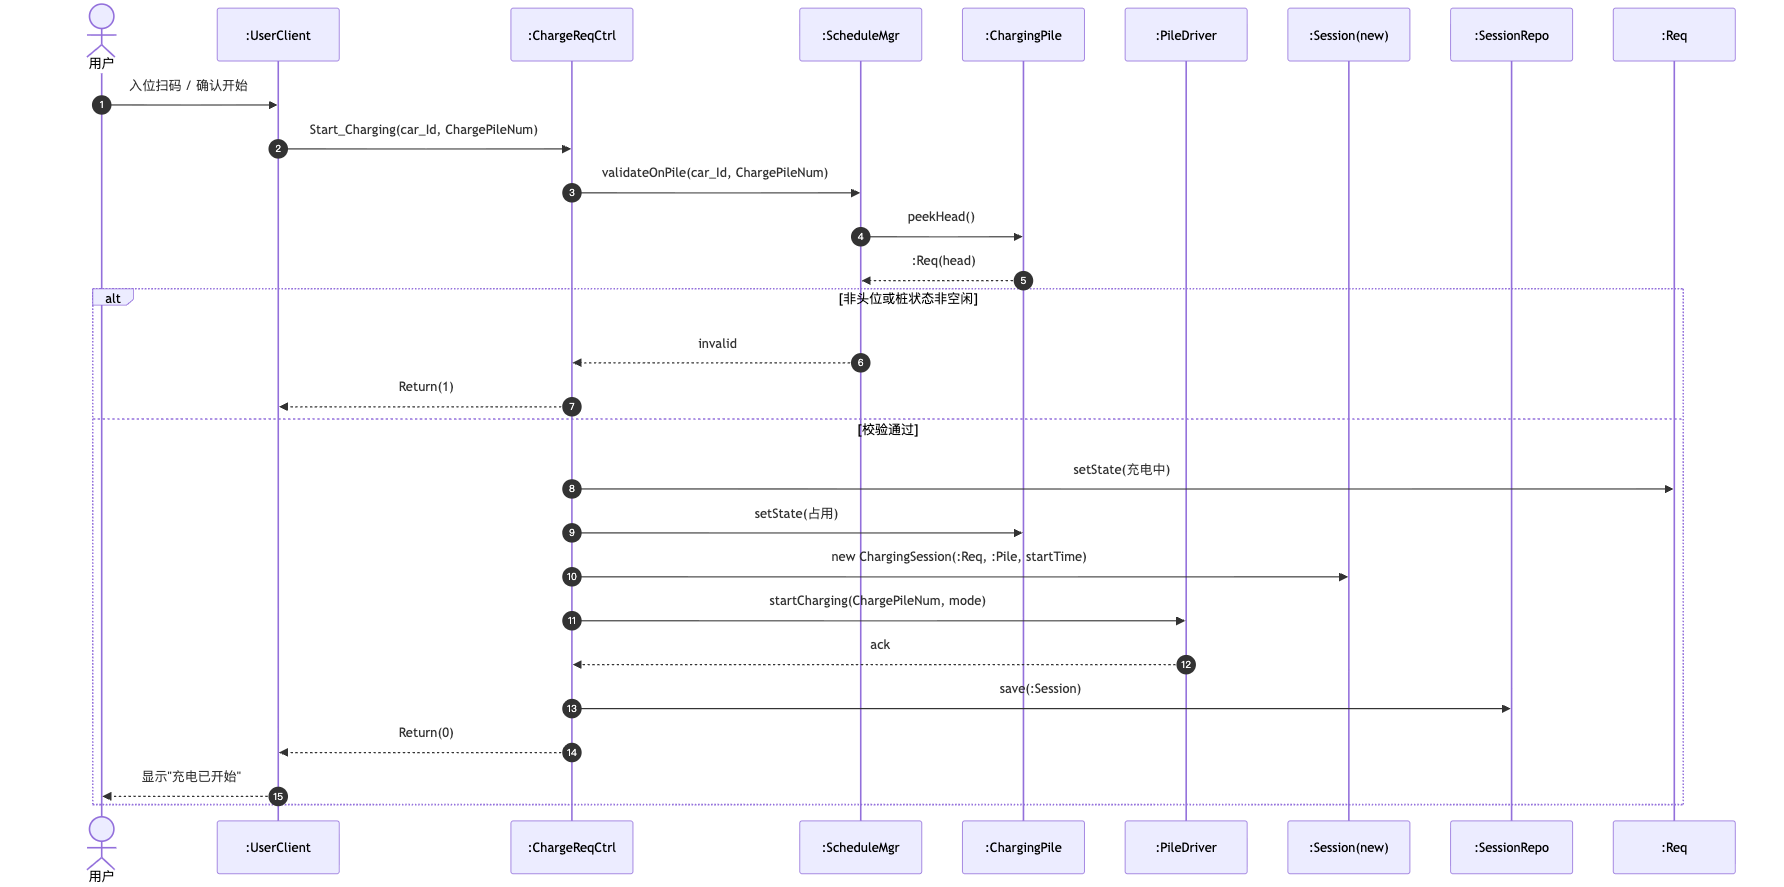
\includegraphics[width=0.95\linewidth]{diagram_06.png}
\end{figure}

\subsubsection{对象设计：Query\_Charging\_State(car\_Id)}

\textbf{(1) 操作契约（已知条件）}

\begin{tabularx}{\linewidth}{p{2.4cm}Y}
\toprule
\textbf{项目} & \textbf{内容} \\
\midrule
系统事件 & \texttt{Query\_Charging\_State(car\_Id)} \\
交叉引用 & UC\_01 充电申请 — 查看充电状态 \\
前置条件 & 1. 当前该车辆存在 \texttt{state=充电中} 的 \texttt{:ChargingSession}。 \\
后置条件 & 1. 从 \texttt{:PileDriver} 拉取实时计量值（累计 kWh、累计时长）。 2. 用当前时刻计算分时电价段 \texttt{chargeRate} 与服务费率 \texttt{serviceRate}。 3. 计算实时费用 \texttt{kWh * (chargeRate + serviceRate)}。 4. 返回详单实时信息（\texttt{pileNum / startTime / kWh / duration / chargeFee / serviceFee / totalFee}）。 5. 不修改持久化业务对象（\texttt{:Session} 只做内存实时刷新）。 \\
\bottomrule
\end{tabularx}

\noindent\textbf{(2) 问题与解决方案}

\begin{tabularx}{\linewidth}{p{5cm}Y}
\toprule
\textbf{问题} & \textbf{解决方案} \\
\midrule
实时电量从哪里来？ & 从物理桩经 \texttt{:PileDriver.pullRealtime(pileId)} 获取计量，避免依赖客户端上报。 \\
分时电价怎么算？ & \texttt{:PricingRule.rateAt(now)} 返回当前时段电价；服务费固定由 \texttt{:ServiceRule.rate()} 提供。 \\
是否需要持久化？ & 不需要，实时查询只刷新 \texttt{:Session.kwh} 和 \texttt{:Session.duration} 的内存视图，账单要等 \texttt{End\_Charging} 时才生成。 \\
\bottomrule
\end{tabularx}

\textbf{(3) Sequence Diagram}

\begin{figure}[ht]
\centering
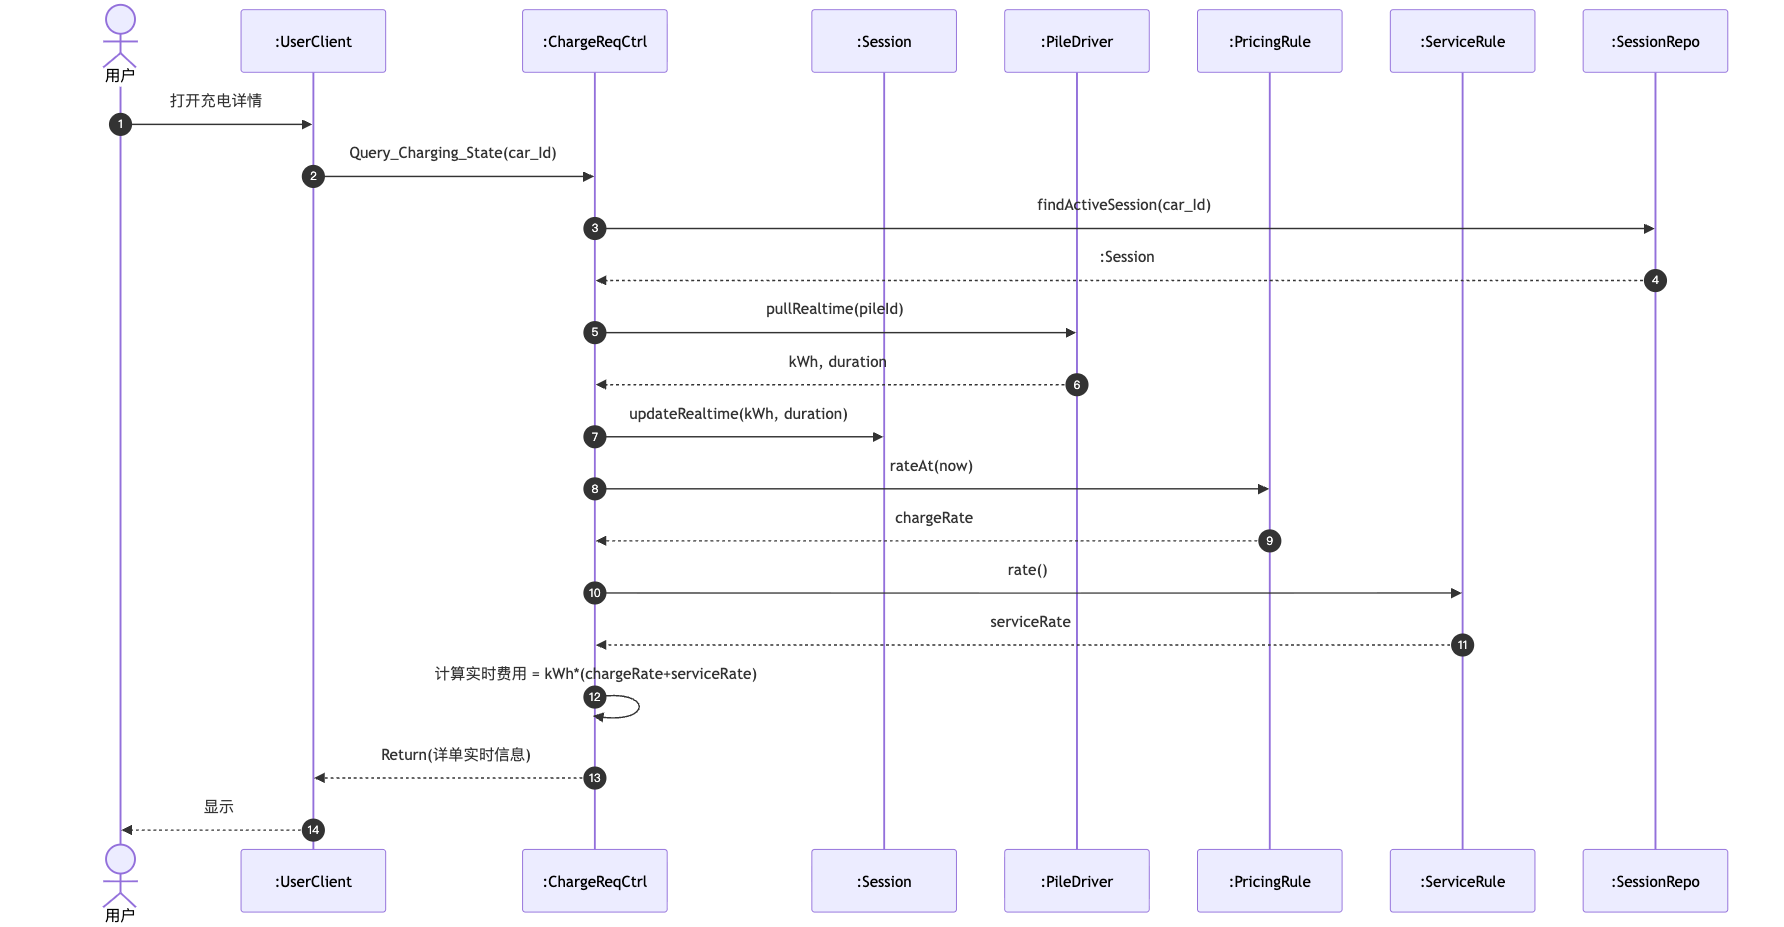
\includegraphics[width=0.95\linewidth]{diagram_07.png}
\end{figure}

\noindent 返回字段按需求说明包含：\texttt{pileNum}、\texttt{startTime}、当前 \texttt{kWh}、当前 \texttt{duration}、估算 \texttt{chargeFee}、估算 \texttt{serviceFee}、当前总费用，与``详单信息''字段一一对应。

\subsubsection{对象设计：End\_Charging(car\_Id, ChargePileNum)}

\textbf{(1) 操作契约（已知条件）}

\begin{tabularx}{\linewidth}{p{2.4cm}Y}
\toprule
\textbf{项目} & \textbf{内容} \\
\midrule
系统事件 & \texttt{End\_Charging(car\_Id, ChargePileNum)} \\
交叉引用 & UC\_01 充电申请 — 结束充电 \\
前置条件 & 1. 该车辆存在 \texttt{state=充电中} 的 \texttt{:Session}，且 \texttt{Session.pileId=ChargePileNum}。 \\
后置条件 & 1. \texttt{:PileDriver.stopCharging(pileId)} 下发停止指令，获取最终 kWh / duration / 分段计量。 2. \texttt{:Session.finalize(kWh, duration, endTime)}，\texttt{:Session.status=COMPLETED}。 3. \texttt{:BillingSvc.generateBill(:Session)} 创建 \texttt{:Bill}。 4. \texttt{:Pile.state=空闲}，立即释放车位，与支付无关。 5. \texttt{:ScheduleMgr.onPileFreed(:Pile)} 触发下一辆调入。 \\
\bottomrule
\end{tabularx}

\noindent\textbf{(2) 问题与解决方案}

\begin{tabularx}{\linewidth}{p{5cm}Y}
\toprule
\textbf{问题} & \textbf{解决方案} \\
\midrule
谁负责生成账单？ & \texttt{:BillingService.generateBill(:Session)} 接受会话对象，依据 \texttt{:PricingRule.ratesBetween(start, end)} 分段计费，再加服务费。 \\
桩何时释放？ & \texttt{:Session.finalize()} 后立刻 \texttt{:Pile.setState(空闲)}，不等支付完成（这是业务规则）。 \\
下一辆怎么调入？ & \texttt{:ScheduleMgr.onPileFreed(:Pile)} 先从桩内排队队列取队首；若桩内为空，再按调度策略从等候区选取。 \\
哪些属性受影响？ & \texttt{:Session.endTime/kWh/duration/status}；\texttt{:Pile.state}；\texttt{:Req.state} 改为``已完成''；新生 \texttt{:Bill.totalFee/payState}。 \\
\bottomrule
\end{tabularx}

\textbf{(3) Sequence Diagram}

\begin{figure}[ht]
\centering
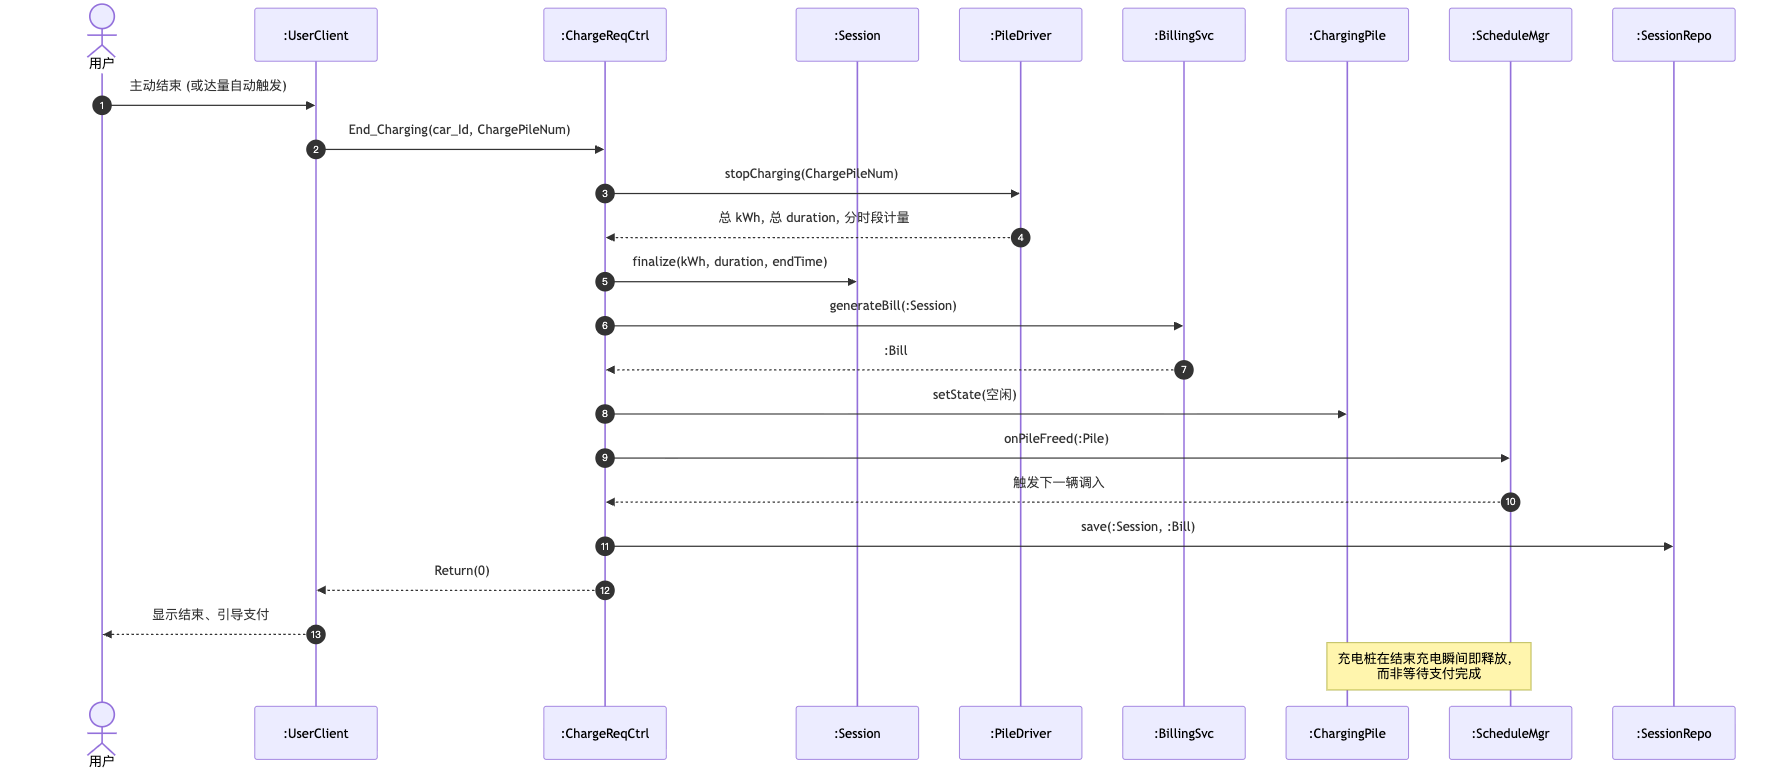
\includegraphics[width=0.95\linewidth]{diagram_08.png}
\end{figure}

\clearpage
%==========================================================
\subsection{用例：查看账单 / 查看详单}

\subsubsection{已知条件}

本用例下系统事件及返回值如下表，每个事件对应的操作契约在下文``对象设计''小节里作为已知条件给出。

\begin{longtable}{p{0.6cm}p{2.4cm}p{6cm}p{6.5cm}}
\toprule
\textbf{序号} & \textbf{指令} & \textbf{系统事件} & \textbf{返回} \\
\midrule
\endhead
1 & 查看账单申请 & \texttt{Request\_Bill(carId, date)} & \texttt{Return(carId, date, Bill\_Id, ChargePileNum, ChargeAmount, ChargeDuration, StartTime, EndTime, TotalChargeFee, TotalServiceFee, TotalFee)} \\
2 & 查看详单申请（子） & \texttt{Request\_DetailedList(Bill\_Id)} & \texttt{Return(carId, date, Bill\_Id, ChargePileNum, ChargeAmount, ChargeDuration, StartTime, EndTime, ChargeFee, ServiceFee, subtotalFee)} \\
\bottomrule
\end{longtable}

\subsubsection{对象设计：Request\_Bill(carId, date)}

\textbf{(1) 操作契约（已知条件）}

\begin{tabularx}{\linewidth}{p{2.4cm}Y}
\toprule
\textbf{项目} & \textbf{内容} \\
\midrule
系统事件 & \texttt{Request\_Bill(carId, date)} \\
交叉引用 & UC\_02 查看账单 — 查看账单申请 \\
前置条件 & 1. 用户身份合法。 2. 查询日期 \texttt{date} 不晚于当日。 \\
后置条件 & 1. 读取该车 \texttt{carId} 在 \texttt{date} 当天结束的全部 \texttt{:Session} 所对应的 \texttt{:Bill} 集合。 2. 按 \texttt{ChargeAmount / Duration / TotalChargeFee / TotalServiceFee / TotalFee} 累加形成汇总账单视图。 3. 不修改任何持久化业务对象，仅返回视图。 \\
\bottomrule
\end{tabularx}

\noindent\textbf{(2) 问题与解决方案}

\begin{tabularx}{\linewidth}{p{5cm}Y}
\toprule
\textbf{问题} & \textbf{解决方案} \\
\midrule
谁负责接收该消息？ & \texttt{:BillController} 作为账单/详单用例的边界。 \\
谁负责聚合？ & \texttt{:BillingService.aggregateBills(carId, date)} 由 \texttt{:BillRepo.findByCarAndDate} 拿到列表后逐条累加。 \\
返回 \texttt{Bill\_Id} 在汇总场景下含义？ & 若当日只有 1 条账单则返回该 \texttt{Bill\_Id}；多条时返回 \texttt{Bill\_Id*} 列表，便于用户进入``详单''页。 \\
\bottomrule
\end{tabularx}

\textbf{(3) Sequence Diagram}

\begin{figure}[ht]
\centering
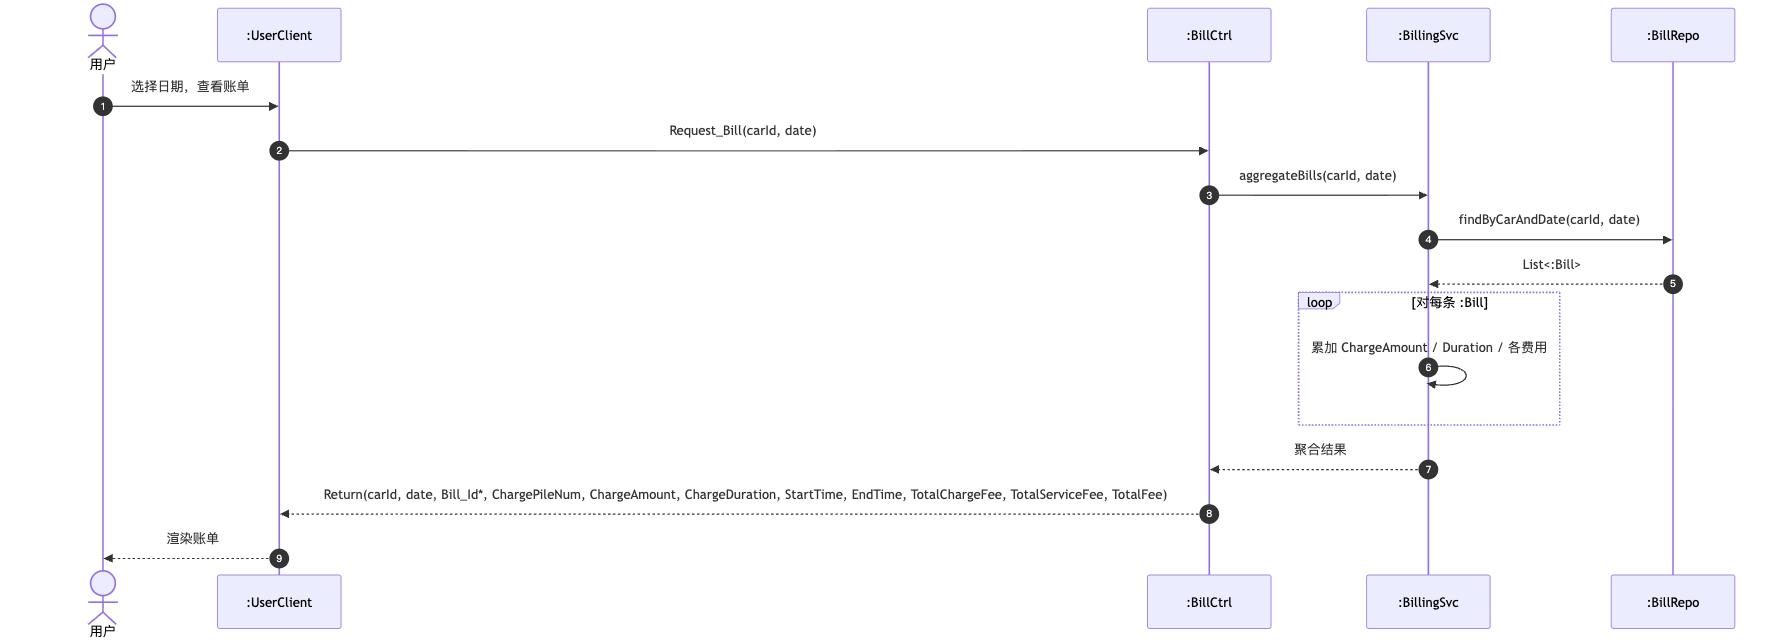
\includegraphics[width=0.9\linewidth]{diagram_09.png}
\end{figure}

\subsubsection{对象设计：Request\_DetailedList(Bill\_Id)}

\textbf{(1) 操作契约（已知条件）}

\begin{tabularx}{\linewidth}{p{2.4cm}Y}
\toprule
\textbf{项目} & \textbf{内容} \\
\midrule
系统事件 & \texttt{Request\_DetailedList(Bill\_Id)} \\
交叉引用 & UC\_02 查看账单（子） — 查看详单申请 \\
前置条件 & 1. \texttt{Bill\_Id} 存在且属于当前用户。 \\
后置条件 & 1. 读取 \texttt{:Bill} 及其 \texttt{:Session}。 2. 通过 \texttt{:PricingRule.ratesBetween(startTime, endTime)} 与 \texttt{:ServiceRule.rate()} 计算分时段的 \texttt{ChargeFee / ServiceFee / subtotalFee}。 3. 返回详单字段。 4. 不修改持久化业务对象。 \\
\bottomrule
\end{tabularx}

\noindent\textbf{(2) 问题与解决方案}

\begin{tabularx}{\linewidth}{p{5cm}Y}
\toprule
\textbf{问题} & \textbf{解决方案} \\
\midrule
详单数据从哪里来？ & 已持久化的 \texttt{:Bill} 提供合计信息；明细分段需要再调一次 \texttt{:PricingRule} 还原。 \\
谁负责生成分段明细？ & \texttt{:BillingService.explodeDetail(:Bill, rates)} 在内存中按电价时段拆分，不写回数据库。 \\
\bottomrule
\end{tabularx}

\textbf{(3) Sequence Diagram}

\begin{figure}[ht]
\centering
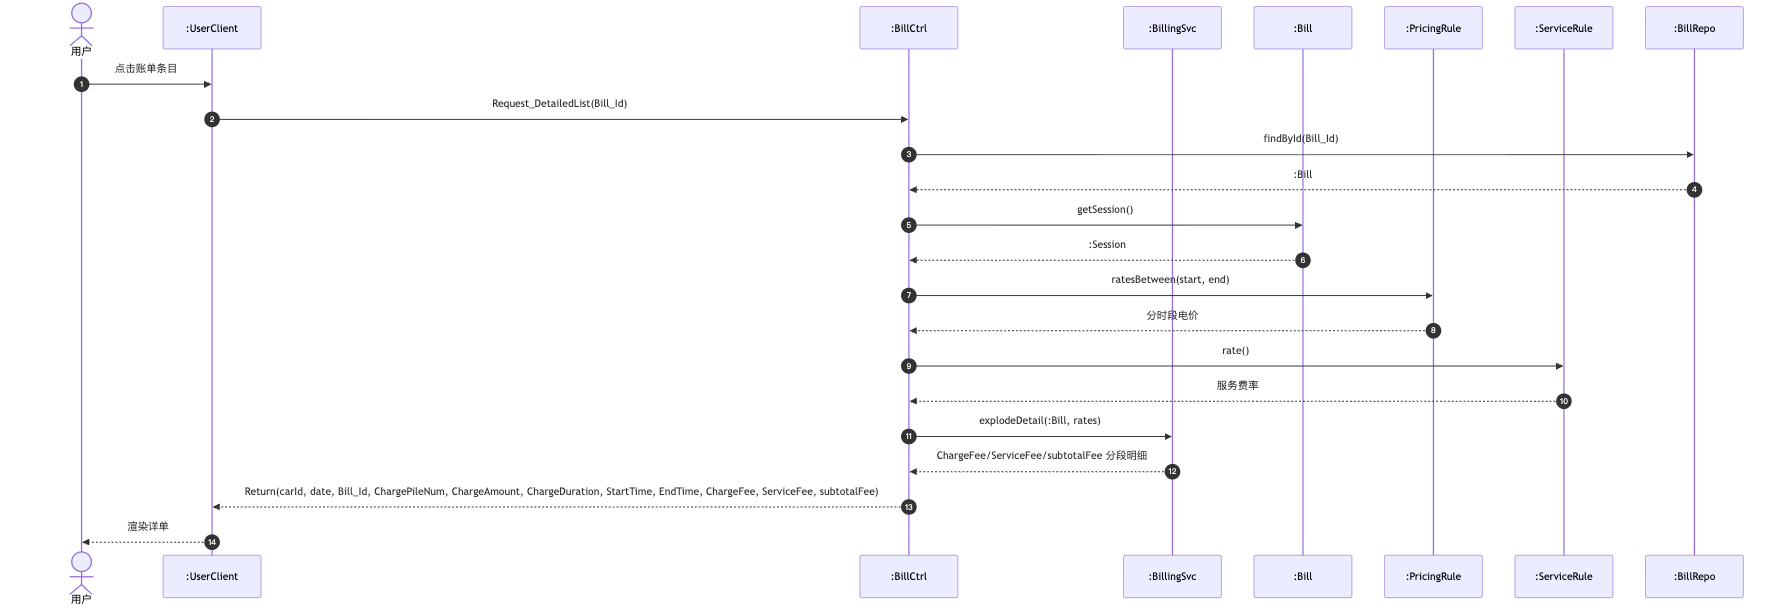
\includegraphics[width=0.95\linewidth]{diagram_10.png}
\end{figure}

\clearpage
%==========================================================
\subsection{用例：运行充电桩}

\subsubsection{已知条件}

\begin{longtable}{cp{2.4cm}p{8cm}p{3cm}}
\toprule
\textbf{序号} & \textbf{指令} & \textbf{系统事件} & \textbf{返回} \\
\midrule
\endhead
1 & 启动充电桩 & \texttt{powerOn(pile\_Id)} & \texttt{Return(0/1)} \\
2 & 设置参数 & \texttt{setParameters(计费规则, 三个时段的电价数据等)} & \texttt{Return(0/1)} \\
3 & 运行充电桩 & \texttt{Start\_ChargingPile(pile\_Id)} & \texttt{Return(0/1)} \\
4 & 关闭充电桩 & \texttt{powerOff(pile\_Id)} & \texttt{Return(0/1)} \\
\bottomrule
\end{longtable}

\subsubsection{对象设计：powerOn(pile\_Id)}

\textbf{(1) 操作契约（已知条件）}

\begin{tabularx}{\linewidth}{p{2.4cm}Y}
\toprule
\textbf{项目} & \textbf{内容} \\
\midrule
系统事件 & \texttt{powerOn(pile\_Id)} \\
交叉引用 & UC\_03 运行充电桩 — 启动充电桩 \\
前置条件 & 1. 管理员身份合法。 2. \texttt{:ChargingPile} 存在且当前状态为``未通电/关闭''。 \\
后置条件 & 1. \texttt{:PileDriver.powerOn(pile\_Id)} 给物理桩供电。 2. \texttt{:Pile.state=待运行}。 3. \texttt{:PileRepo} 持久化新状态。 \\
\bottomrule
\end{tabularx}

\noindent\textbf{(2) 问题与解决方案}

\begin{tabularx}{\linewidth}{p{5cm}Y}
\toprule
\textbf{问题} & \textbf{解决方案} \\
\midrule
谁负责接收该消息？ & \texttt{:PileController} 作为管理员侧充电桩用例的边界。 \\
是否直接操作硬件？ & 否。控制器把请求转给 \texttt{:PileService.powerOn(pile\_Id)}，由后者经 \texttt{:PileDriver} 下发。 \\
哪些属性需要修改？ & \texttt{:Pile.state} 从``未通电''改为``待运行''；其余统计字段不变。 \\
\bottomrule
\end{tabularx}

\textbf{(3) Sequence Diagram}

\begin{figure}[ht]
\centering
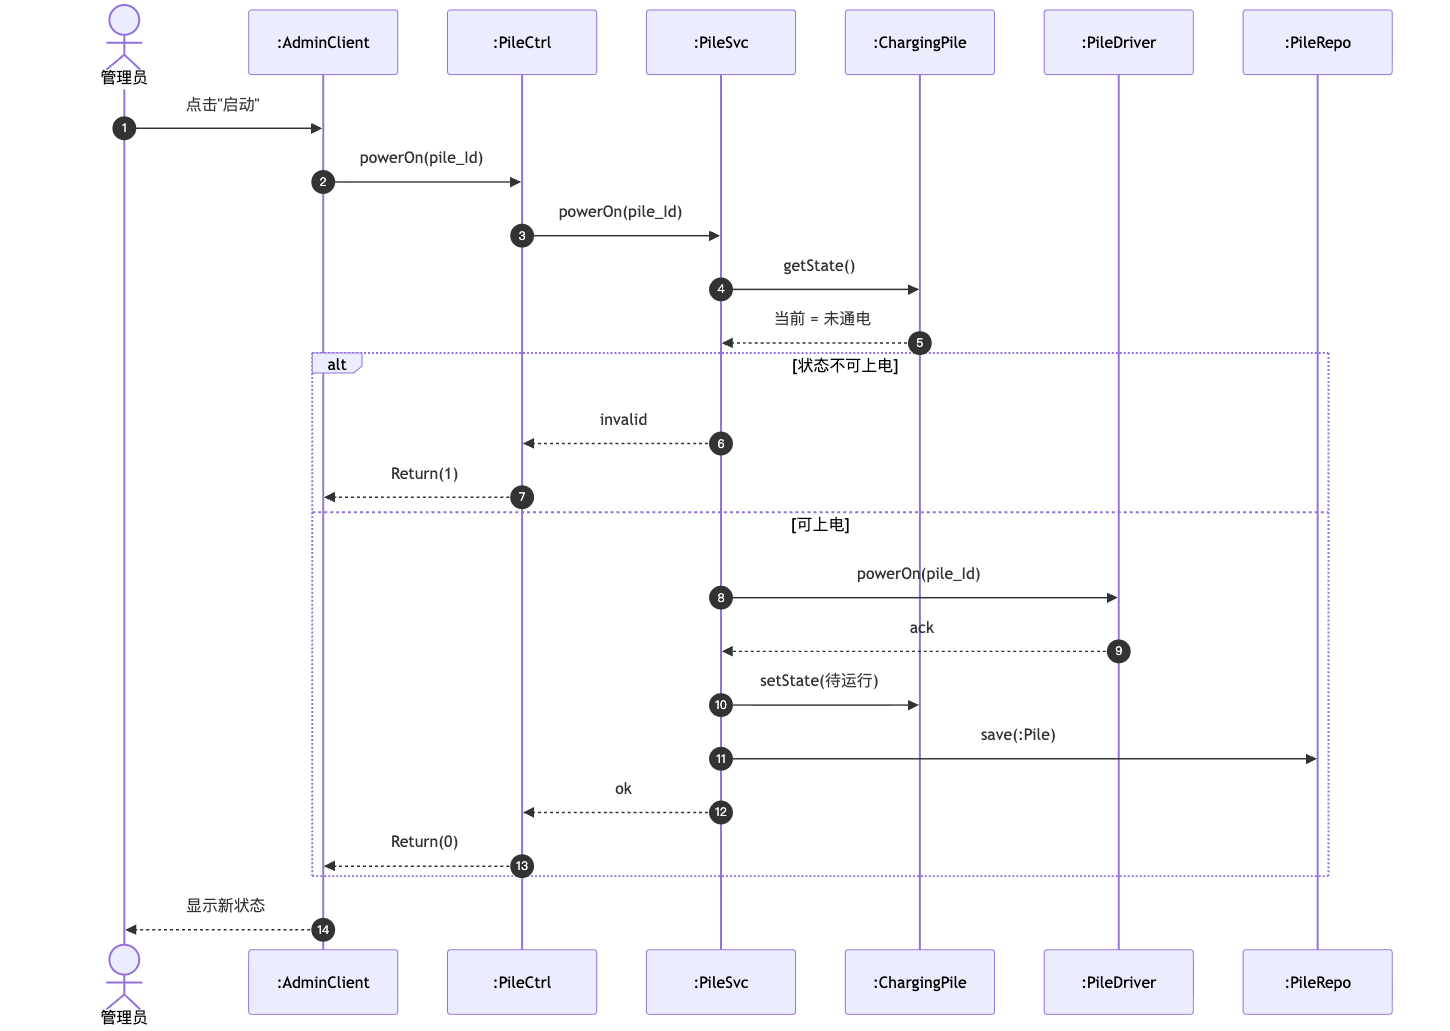
\includegraphics[width=0.9\linewidth]{diagram_11.png}
\end{figure}

\subsubsection{对象设计：setParameters(计费规则, 三个时段的电价数据等)}

\textbf{(1) 操作契约（已知条件）}

\begin{tabularx}{\linewidth}{p{2.4cm}Y}
\toprule
\textbf{项目} & \textbf{内容} \\
\midrule
系统事件 & \texttt{setParameters(billingRule, peakRate, normalRate, valleyRate, serviceRate)} \\
交叉引用 & UC\_03 运行充电桩 — 设置参数 \\
前置条件 & 1. 管理员身份合法。 2. 三个时段电价和服务费率均 \texttt{> 0}。 \\
后置条件 & 1. 更新 \texttt{:PricingRule.\{peakRate, normalRate, valleyRate\}}、\texttt{:ServiceRule.rate}、\texttt{validFrom=now}。 2. 通过 \texttt{:PileDriver.pushParam} 把新参数下发到所有运行中的 5 个 \texttt{:ChargingPile}。 3. 持久化到 \texttt{:PriceRepo}。 \\
\bottomrule
\end{tabularx}

\noindent\textbf{(2) 问题与解决方案}

\begin{tabularx}{\linewidth}{p{5cm}Y}
\toprule
\textbf{问题} & \textbf{解决方案} \\
\midrule
价格对象更新策略？ & 不在原对象上原地改值，而是 \texttt{:PricingRule.update(...)} 内部创建一条新版本记录，方便回溯历史账单分段计费。 \\
5 个桩如何同步？ & 在 \texttt{:PileService.applyParameters} 内部用 \texttt{par} 并行块向 5 个 \texttt{:PileDriver} 端点下发 \texttt{pushParam}。 \\
是否影响在充会话？ & 仅影响 \texttt{validFrom} 之后开始的会话；当前在充会话仍按其会话开始时的电价时段表计费，以维持历史一致性。 \\
\bottomrule
\end{tabularx}

\textbf{(3) Sequence Diagram}

\begin{figure}[ht]
\centering
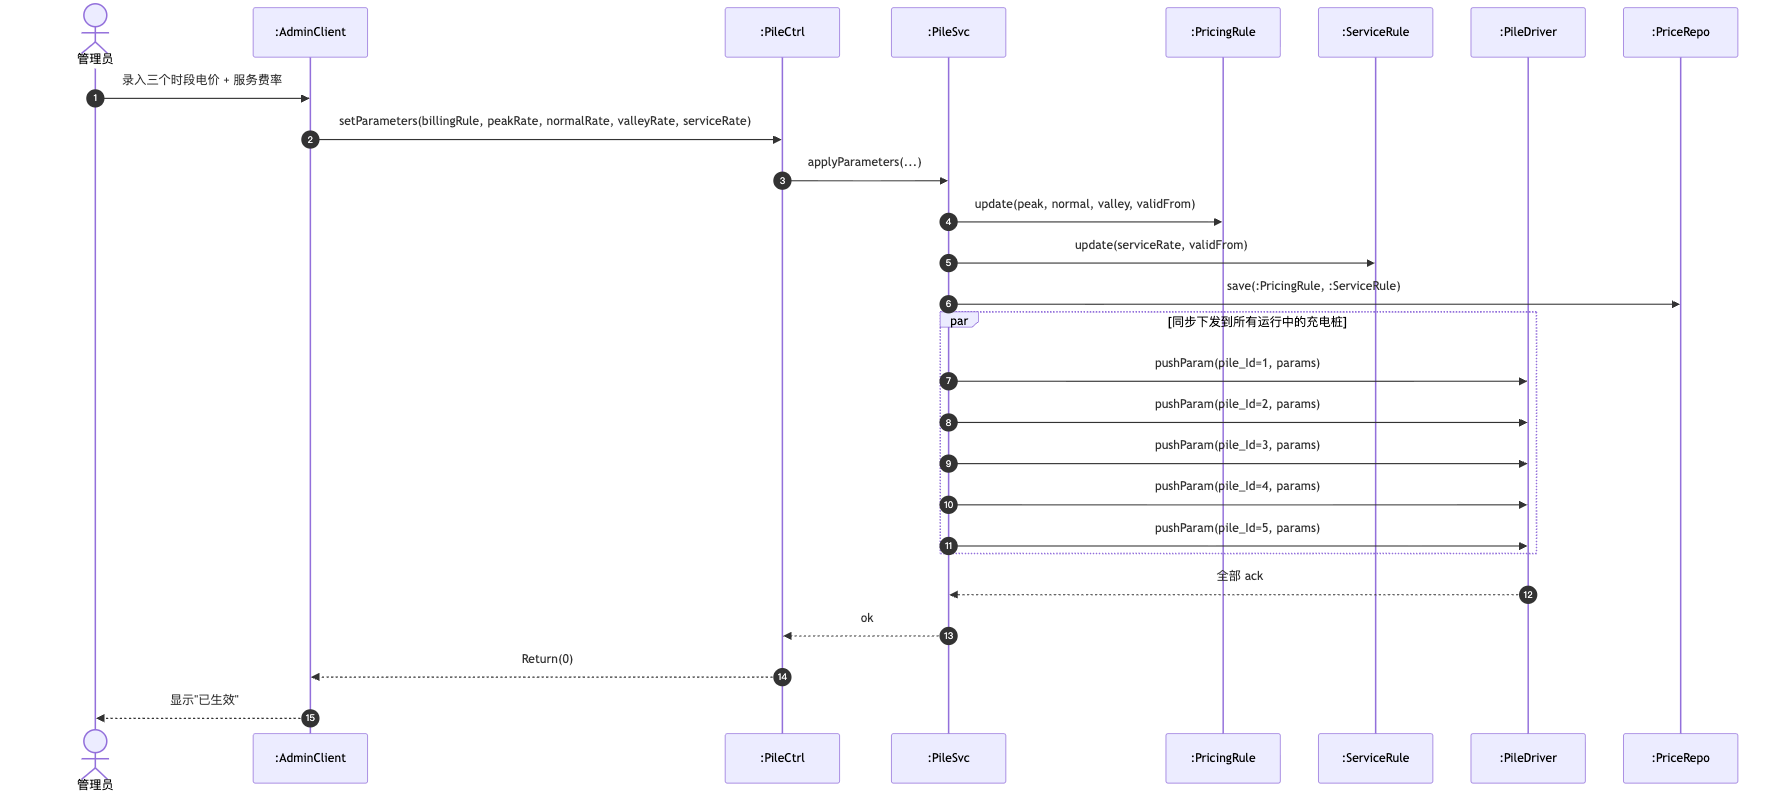
\includegraphics[width=0.95\linewidth]{diagram_12.png}
\end{figure}

\subsubsection{对象设计：Start\_ChargingPile(pile\_Id)}

\textbf{(1) 操作契约（已知条件）}

\begin{tabularx}{\linewidth}{p{2.4cm}Y}
\toprule
\textbf{项目} & \textbf{内容} \\
\midrule
系统事件 & \texttt{Start\_ChargingPile(pile\_Id)} \\
交叉引用 & UC\_03 运行充电桩 — 运行充电桩 \\
前置条件 & 1. \texttt{:Pile.state=待运行}（即已 \texttt{powerOn} 但尚未投入服务）。 \\
后置条件 & 1. \texttt{:PileDriver.startService(pile\_Id)} 进入对外服务模式。 2. \texttt{:Pile.state=空闲}。 3. \texttt{:ScheduleMgr.registerAvailable(:Pile)} 触发调度入队；若同模式 \texttt{:WaitingQueue} 有等待车辆，立即开始调入。 \\
\bottomrule
\end{tabularx}

\noindent\textbf{(2) 问题与解决方案}

\begin{tabularx}{\linewidth}{p{5cm}Y}
\toprule
\textbf{问题} & \textbf{解决方案} \\
\midrule
谁向调度器宣告``新桩可用''？ & \texttt{:PileService.start} 完成后调用 \texttt{:ScheduleMgr.registerAvailable(:Pile)}。 \\
状态校验失败如何处理？ & 直接返回 \texttt{1}（例如未通电先调用本指令则拒绝）。 \\
与 \texttt{powerOn} 的区别？ & \texttt{powerOn} 只给桩通电、让桩自检；\texttt{Start\_ChargingPile} 才真正接入调度，开始接受调入。 \\
\bottomrule
\end{tabularx}

\textbf{(3) Sequence Diagram}

\begin{figure}[ht]
\centering
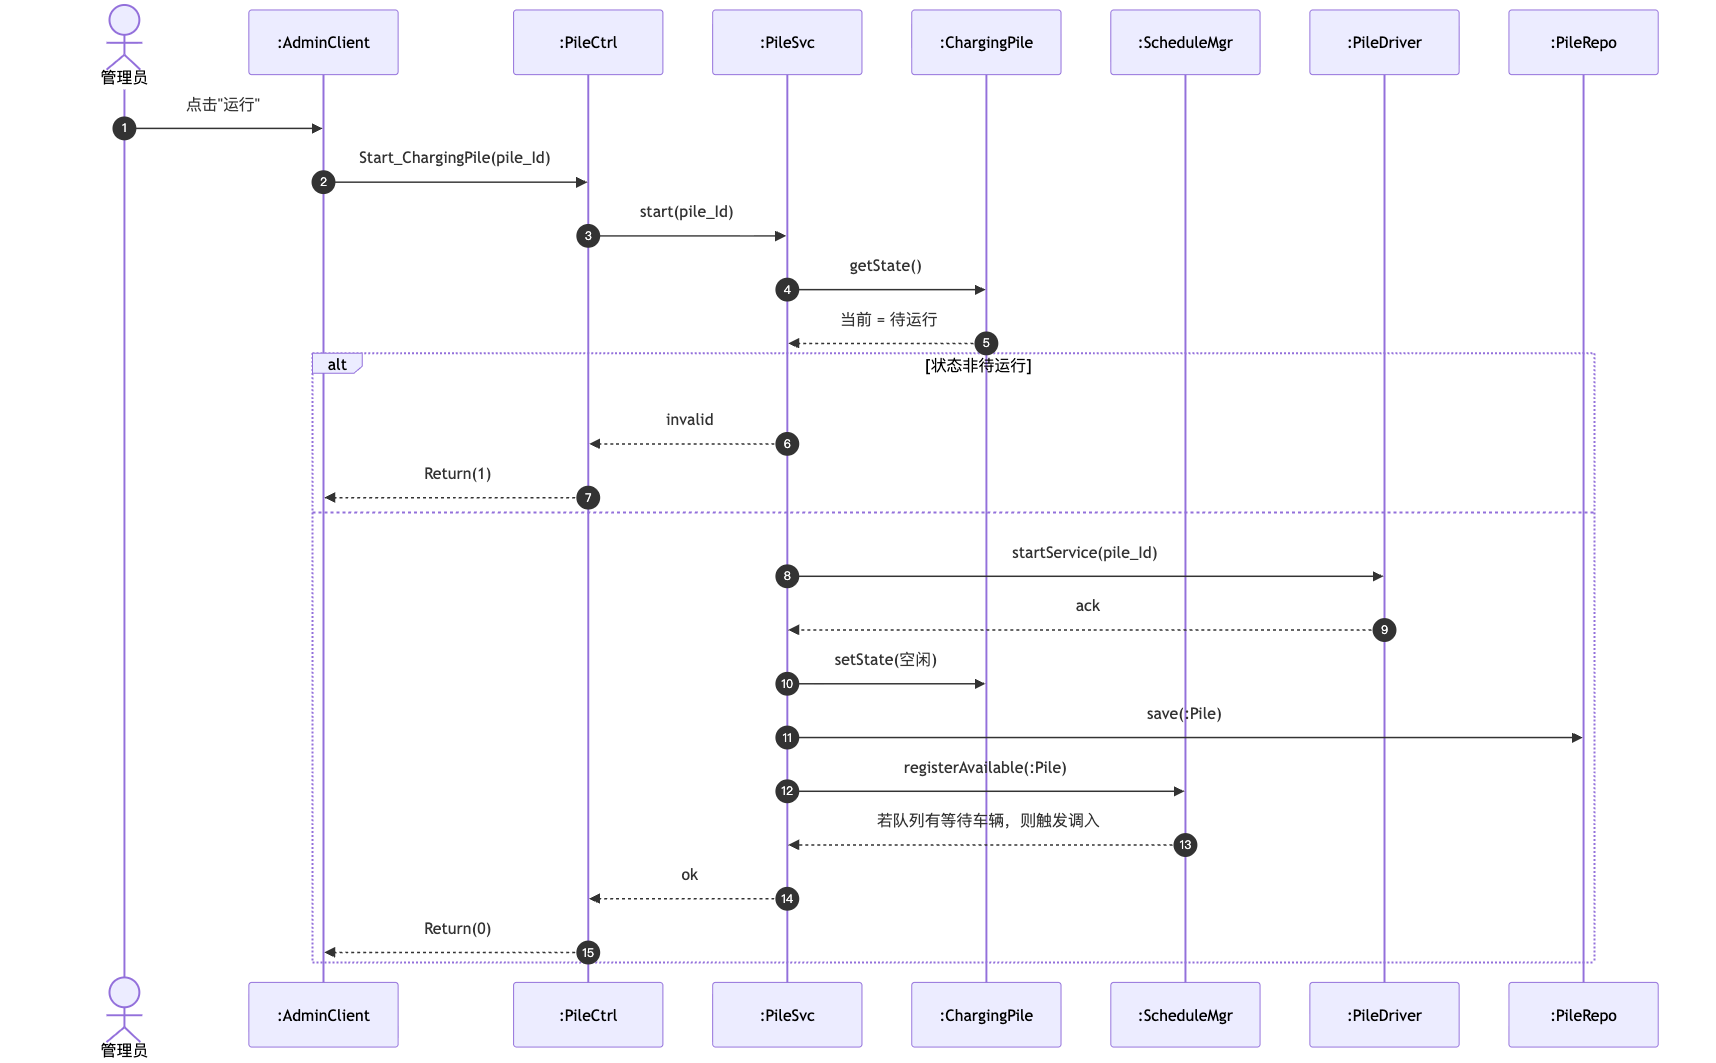
\includegraphics[width=0.9\linewidth]{diagram_13.png}
\end{figure}

\subsubsection{对象设计：powerOff(pile\_Id)}

\textbf{(1) 操作契约（已知条件）}

\begin{tabularx}{\linewidth}{p{2.4cm}Y}
\toprule
\textbf{项目} & \textbf{内容} \\
\midrule
系统事件 & \texttt{powerOff(pile\_Id)} \\
交叉引用 & UC\_03 运行充电桩 — 关闭充电桩 \\
前置条件 & 1. \texttt{:Pile} 存在。 \\
后置条件 & 1. 若该桩当前正在为某辆车充电，先 \texttt{:Session.finalize(snapshot)} 并由 \texttt{:BillingSvc.generateBill} 出阶段账单。 2. 桩内排队车辆经 \texttt{:ScheduleMgr.returnWaitersToWaitingArea(:Pile)} 回到等候区。 3. \texttt{:PileDriver.powerOff(pile\_Id)} 物理断电。 4. \texttt{:Pile.state=关闭}，\texttt{:ScheduleMgr.unregisterAvailable(:Pile)} 不再参与调度。 \\
\bottomrule
\end{tabularx}

\noindent\textbf{(2) 问题与解决方案}

\begin{tabularx}{\linewidth}{p{5cm}Y}
\toprule
\textbf{问题} & \textbf{解决方案} \\
\midrule
关闭时是否允许中断在充会话？ & 业务允许：\texttt{:Session} 立即结束并出阶段账单，用户被通知。 \\
桩内排队车辆如何处理？ & 由 \texttt{:ScheduleMgr.returnWaitersToWaitingArea(:Pile)} 把它们以原 \texttt{request\_time} 退回等候区，保持公平。 \\
与故障（FaultService）的区别？ & \texttt{powerOff} 是管理员主动维护，\texttt{onPileFault} 是异常事件；前者不创建 \texttt{:FaultRecord}。 \\
\bottomrule
\end{tabularx}

\textbf{(3) Sequence Diagram}

\begin{figure}[ht]
\centering
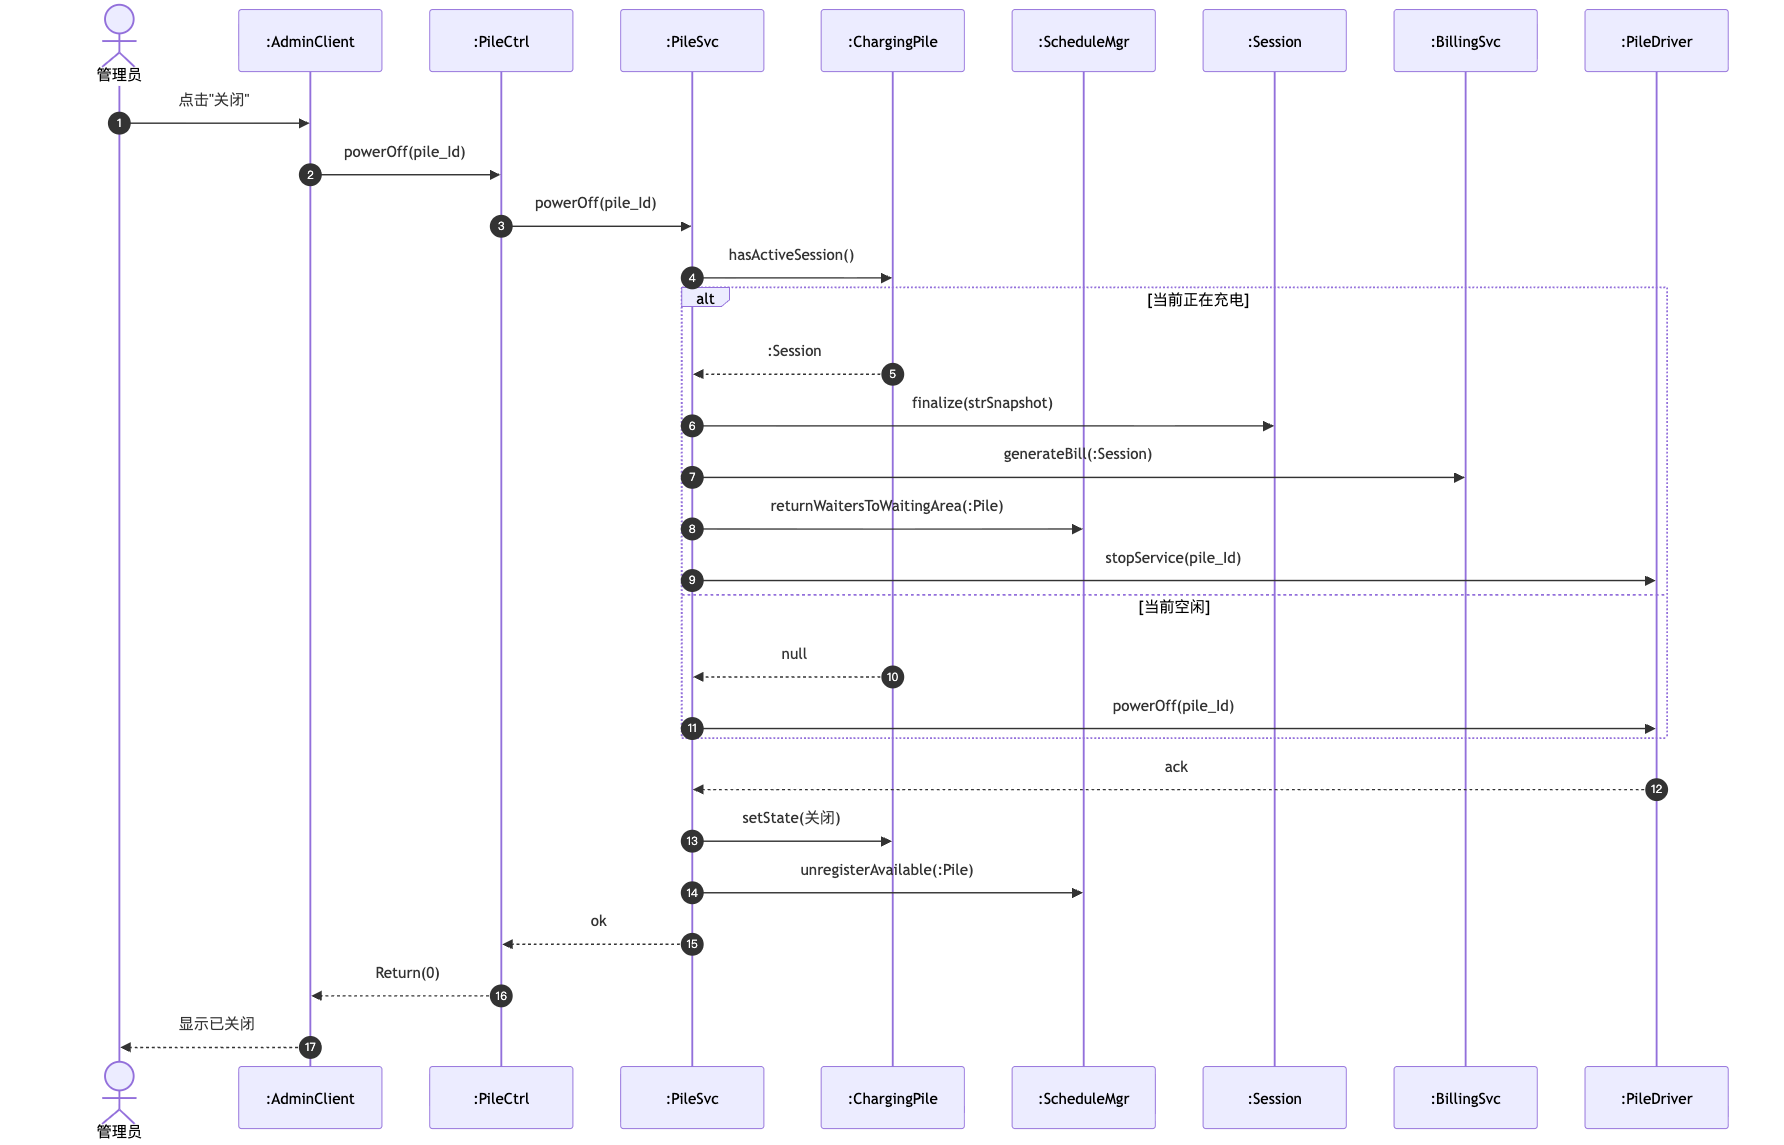
\includegraphics[width=0.95\linewidth]{diagram_14.png}
\end{figure}

\clearpage
%==========================================================
\subsection{用例：查看充电桩状态 / 查看队列状态}

\subsubsection{已知条件}

\begin{longtable}{cp{3.6cm}p{6cm}p{5cm}}
\toprule
\textbf{序号} & \textbf{指令} & \textbf{系统事件} & \textbf{返回} \\
\midrule
\endhead
1 & 查看充电桩状态（定时刷新） & \texttt{Query\_PileState(pile\_Id)} & \texttt{Return(workingState, TotalChargeNum, TotalChargeTime, TotalCapacity)} \\
2 & 查看队列状态（子） & \texttt{Query\_QueueState(queuelist)} & \texttt{Return(car\_Id, car\_Capacity, Request\_Amount, waitTime)} \\
\bottomrule
\end{longtable}

\subsubsection{对象设计：Query\_PileState(pile\_Id)}

\textbf{(1) 操作契约（已知条件）}

\begin{tabularx}{\linewidth}{p{2.4cm}Y}
\toprule
\textbf{项目} & \textbf{内容} \\
\midrule
系统事件 & \texttt{Query\_PileState(pile\_Id)} \\
交叉引用 & UC\_04 查看充电桩状态 \\
前置条件 & 1. 管理员登录。 2. \texttt{:Pile} 存在；\texttt{pile\_Id} 为空表示全量查询（展开为 5 个并行 \texttt{Query\_PileState}）。 \\
后置条件 & 1. 读取 \texttt{:Pile.workingState}。 2. 由 \texttt{:PileDriver.pullCounters} 获取累计 \texttt{TotalChargeNum / TotalChargeTime / TotalCapacity}。 3. \texttt{:PileRepo.snapshot(:Pile)} 写回最新计数（视为副作用，便于运营报表）。 \\
\bottomrule
\end{tabularx}

\noindent\textbf{(2) 问题与解决方案}

\begin{tabularx}{\linewidth}{p{5cm}Y}
\toprule
\textbf{问题} & \textbf{解决方案} \\
\midrule
客户端如何实现定时刷新？ & \texttt{:AdminClient} 内部按 \texttt{refreshInterval=N}（默认 5s）周期调用本接口；服务端不维护推送通道。 \\
5 个桩并发查询如何组织？ & 在 \texttt{:PileController} 内部展开为 5 个并行任务，避免阻塞。 \\
该指令是否修改业务对象？ & 仅写入桩累计计数快照（\texttt{snapshot}），不改变核心状态字段；视为只读 + 计数副作用。 \\
\bottomrule
\end{tabularx}

\textbf{(3) Sequence Diagram}

\begin{figure}[ht]
\centering
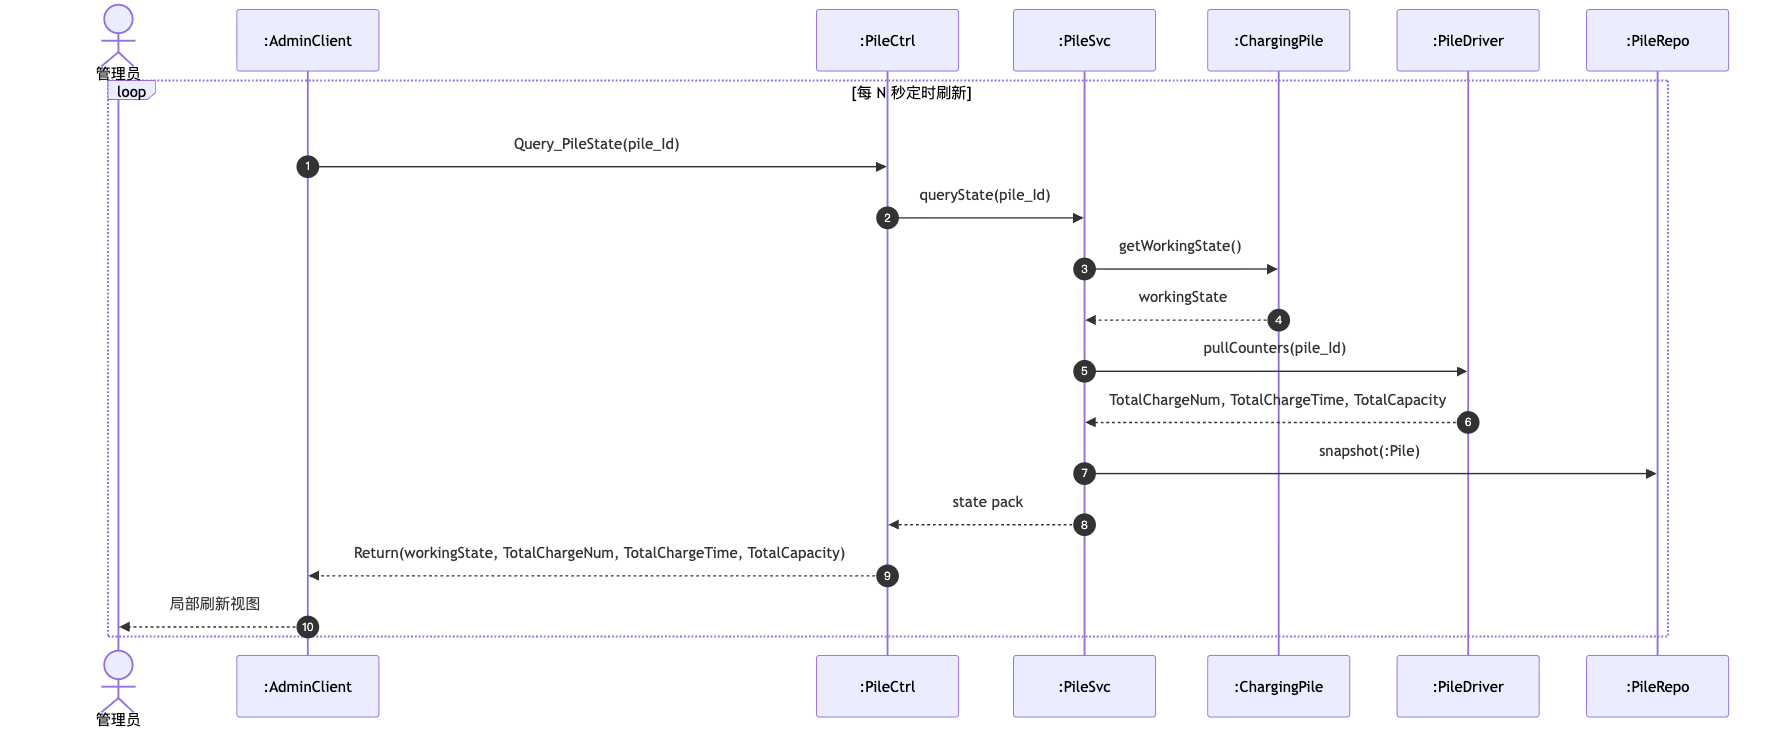
\includegraphics[width=0.95\linewidth]{diagram_15.png}
\end{figure}

\noindent 客户端按 \texttt{N}（默认 5s）周期发起请求；当 \texttt{pile\_Id} 为空时由 \texttt{:PileCtrl} 内部展开为 5 个并行 \texttt{queryState}。

\subsubsection{对象设计：Query\_QueueState(queuelist)}

\textbf{(1) 操作契约（已知条件）}

\begin{tabularx}{\linewidth}{p{2.4cm}Y}
\toprule
\textbf{项目} & \textbf{内容} \\
\midrule
系统事件 & \texttt{Query\_QueueState(queuelist)} \\
交叉引用 & UC\_04 查看队列状态（子） \\
前置条件 & 1. 管理员登录。 2. \texttt{queuelist} 中的每个队列 ID 都存在（等候区 fast/slow，或 5 个桩内队列）。 \\
后置条件 & 1. 对每个队列读取队列中 \texttt{:Req} 列表。 2. 对每个请求估算 \texttt{waitTime}（等待至开始充电的分钟数）。 3. 返回每条记录 \texttt{(car\_Id, car\_Capacity, Request\_Amount, waitTime)}。 4. 不修改持久化业务对象。 \\
\bottomrule
\end{tabularx}

\noindent\textbf{(2) 问题与解决方案}

\begin{tabularx}{\linewidth}{p{5cm}Y}
\toprule
\textbf{问题} & \textbf{解决方案} \\
\midrule
谁负责跨等候区/桩内队列的统一查询？ & \texttt{:QueueController} 调用 \texttt{:ScheduleMgr.snapshot(queueId)}，后者根据 \texttt{queueId} 在 \texttt{:WaitingArea} 与 \texttt{:ChargingArea} 中分发。 \\
\texttt{waitTime} 如何估算？ & 等候区中：排在前面的所有请求充电时长 + 桩平均排队时长；桩内队列：在充会话剩余 + 之前各位等候充电时长。 \\
是否需要锁？ & 不需要。整个查询是只读快照，估算函数容忍短暂的并发漂移。 \\
\bottomrule
\end{tabularx}

\textbf{(3) Sequence Diagram}

\begin{figure}[ht]
\centering
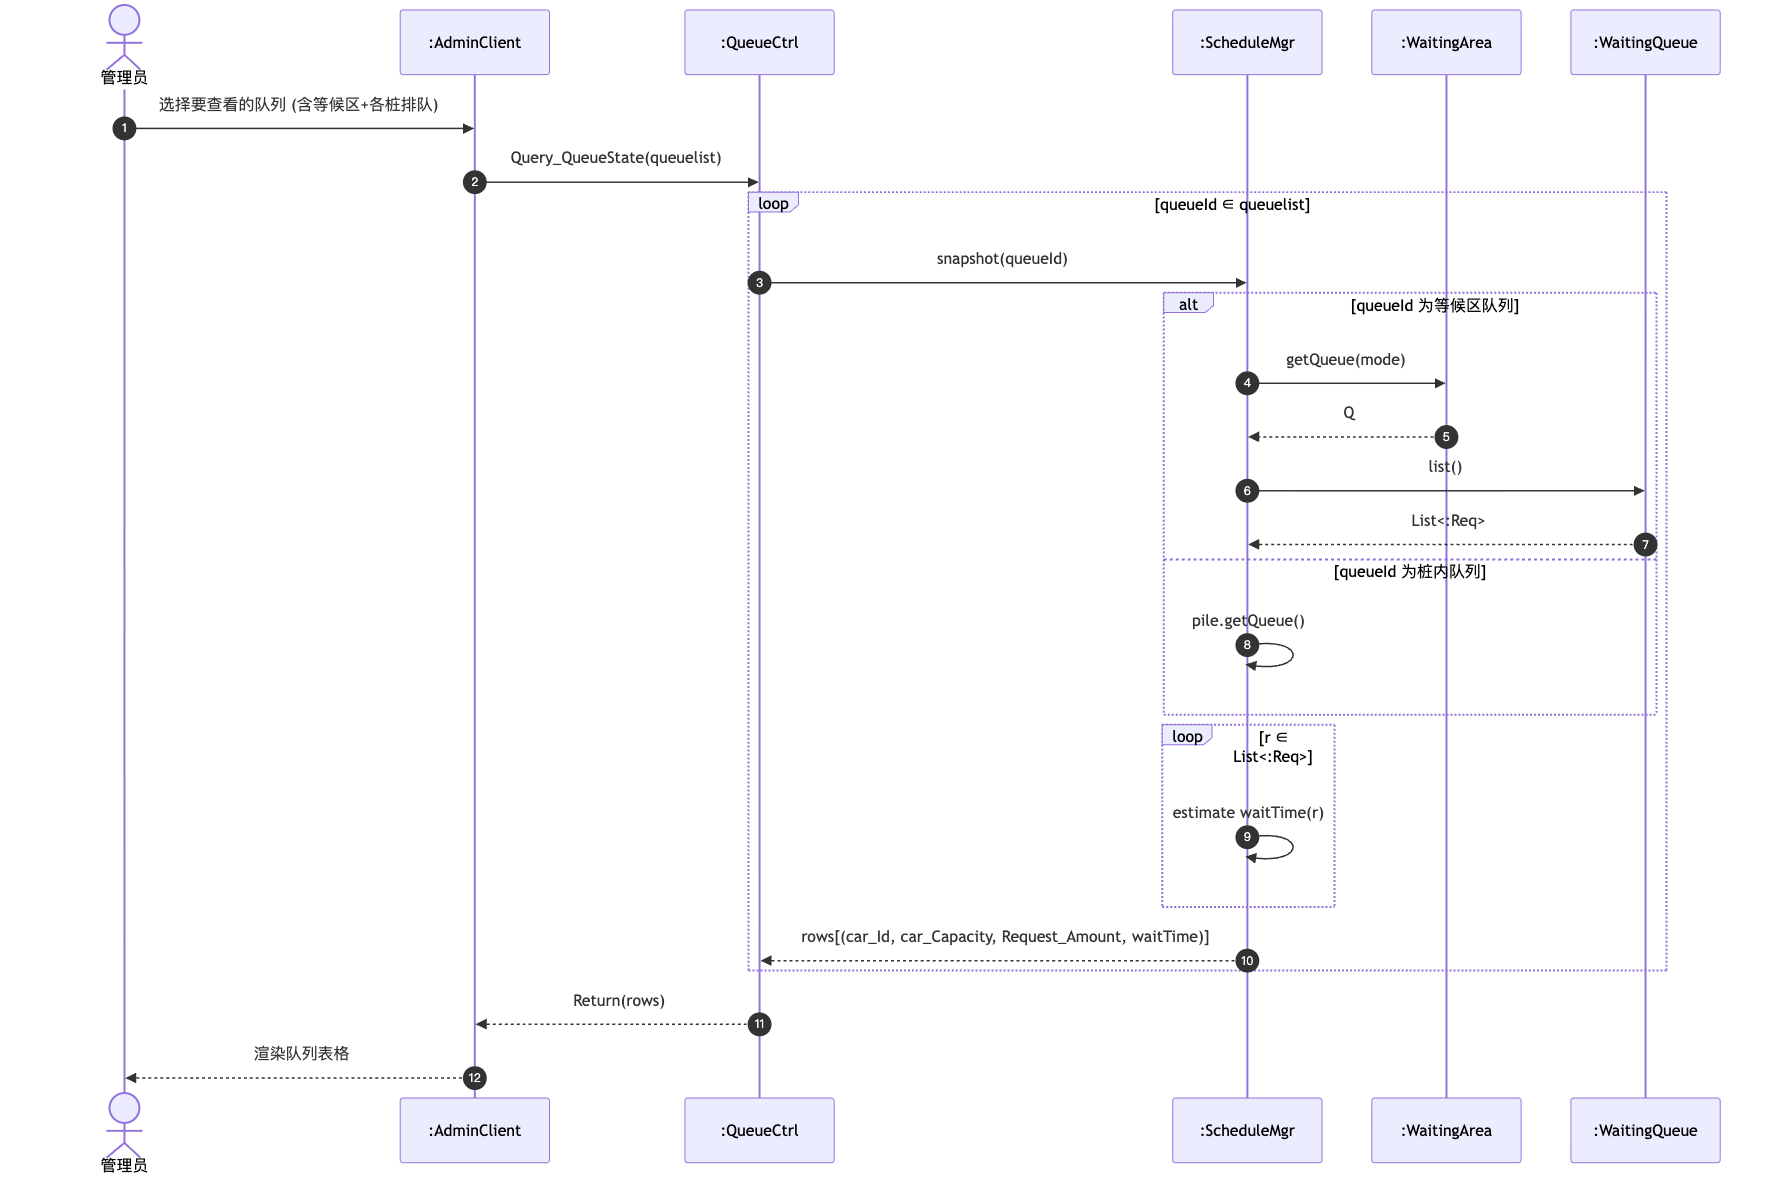
\includegraphics[width=0.95\linewidth]{diagram_16.png}
\end{figure}

\clearpage
%==========================================================
\subsection{用例：调度对象核心交互（组长部分）}

本节由组长唐振桓完成。针对充电过程中出现某个充电桩故障的情况，分别给出 (1) 优先级调度、(2) 时间顺序调度、(3) 充电中故障恢复 三种调度对象之间的交互过程。

\subsubsection{已知条件}

公共前提：5 个充电桩中 \texttt{Pile\_F} 在某辆车 \texttt{Car\_X} 充电过程中发生硬件故障。\texttt{Car\_X} 已充入 \texttt{Δ} 度电、\texttt{Pile\_F} 队尾还排有 \texttt{Car\_Y}（尚未开始充电）。下文三张图分别采用不同的``再调度''策略来处理。

参与调度的对象与外部消息如下：

\begin{longtable}{p{0.6cm}p{2.8cm}p{6cm}p{6cm}}
\toprule
\textbf{序号} & \textbf{事件} & \textbf{调度交互} & \textbf{输出} \\
\midrule
\endhead
1 & 优先级调度 & \texttt{onPileFault(pile\_F)}，保留 \texttt{Car\_X} 原优先级直接调入同模式空闲桩 & \texttt{dispatchNotify(Car\_X, Pile\_Other)} \\
2 & 时间顺序调度 & \texttt{onPileFault(pile\_F)}，把 \texttt{Car\_X / Car\_Y} 都按原 \texttt{request\_time} 退回等待队列 & 按新 FIFO 通知队首车辆 \\
3 & 充电中故障恢复 & \texttt{ResumePile(pile\_F)} 后重新参与同模式调度 & \texttt{dispatchNotify(:Req(head), :Pile\_F)} \\
\bottomrule
\end{longtable}

操作契约（合并表述以避免重复）：

\begin{tabularx}{\linewidth}{p{2.6cm}Y}
\toprule
\textbf{项目} & \textbf{内容} \\
\midrule
系统事件 & \texttt{onPileFault(pile\_F)}（由 \texttt{:PileDriver} 异步告警触发）和 \texttt{ResumePile(pile\_F)} \\
交叉引用 & UC\_03/UC\_04 调度对象核心交互 \\
前置条件 & 1. \texttt{Pile\_F} 正处于服务中或被告警检测到硬件异常。 2. 故障告警进入 \texttt{:FaultSvc}。 \\
后置条件（故障） & 1. \texttt{:Pile\_F.state=故障中}。 2. 在充会话 \texttt{:Session(Car\_X)} 立即 \texttt{stopMeter} 并出阶段账单。 3. 创建续充 \texttt{:Req(Car\_X 续充)}，按策略（优先级 / 时间顺序）加入同模式等待队列或直接调入空闲桩。 4. 桩内未开始的请求（\texttt{Car\_Y}）按策略退回等待队列。 \\
后置条件（恢复） & 1. \texttt{:Pile\_F.state=空闲}，\texttt{:FaultRecord.close()}。 2. \texttt{:ScheduleMgr.registerAvailable(:Pile\_F)} 触发同模式调入。 3. 把``故障中断''会话的快照费用合并到主账单。 \\
\bottomrule
\end{tabularx}

\subsubsection{对象设计：优先级调度}

\textbf{问题与解决方案}

\begin{tabularx}{\linewidth}{p{5.4cm}Y}
\toprule
\textbf{问题} & \textbf{解决方案} \\
\midrule
\texttt{Car\_X} 续充请求是否需要重新排队？ & 不需要：复用其原 \texttt{request\_time}，确保位于所有同模式新车之前。 \\
谁负责``绕过等待区直接进入空闲桩''？ & \texttt{:ScheduleMgr} 在收到 \texttt{:FaultSvc} 通知后，立刻在同模式 \texttt{:Pile\_Other} 中找空位；有则直接 enqueue。 \\
\bottomrule
\end{tabularx}

\textbf{Sequence Diagram}

\begin{figure}[ht]
\centering
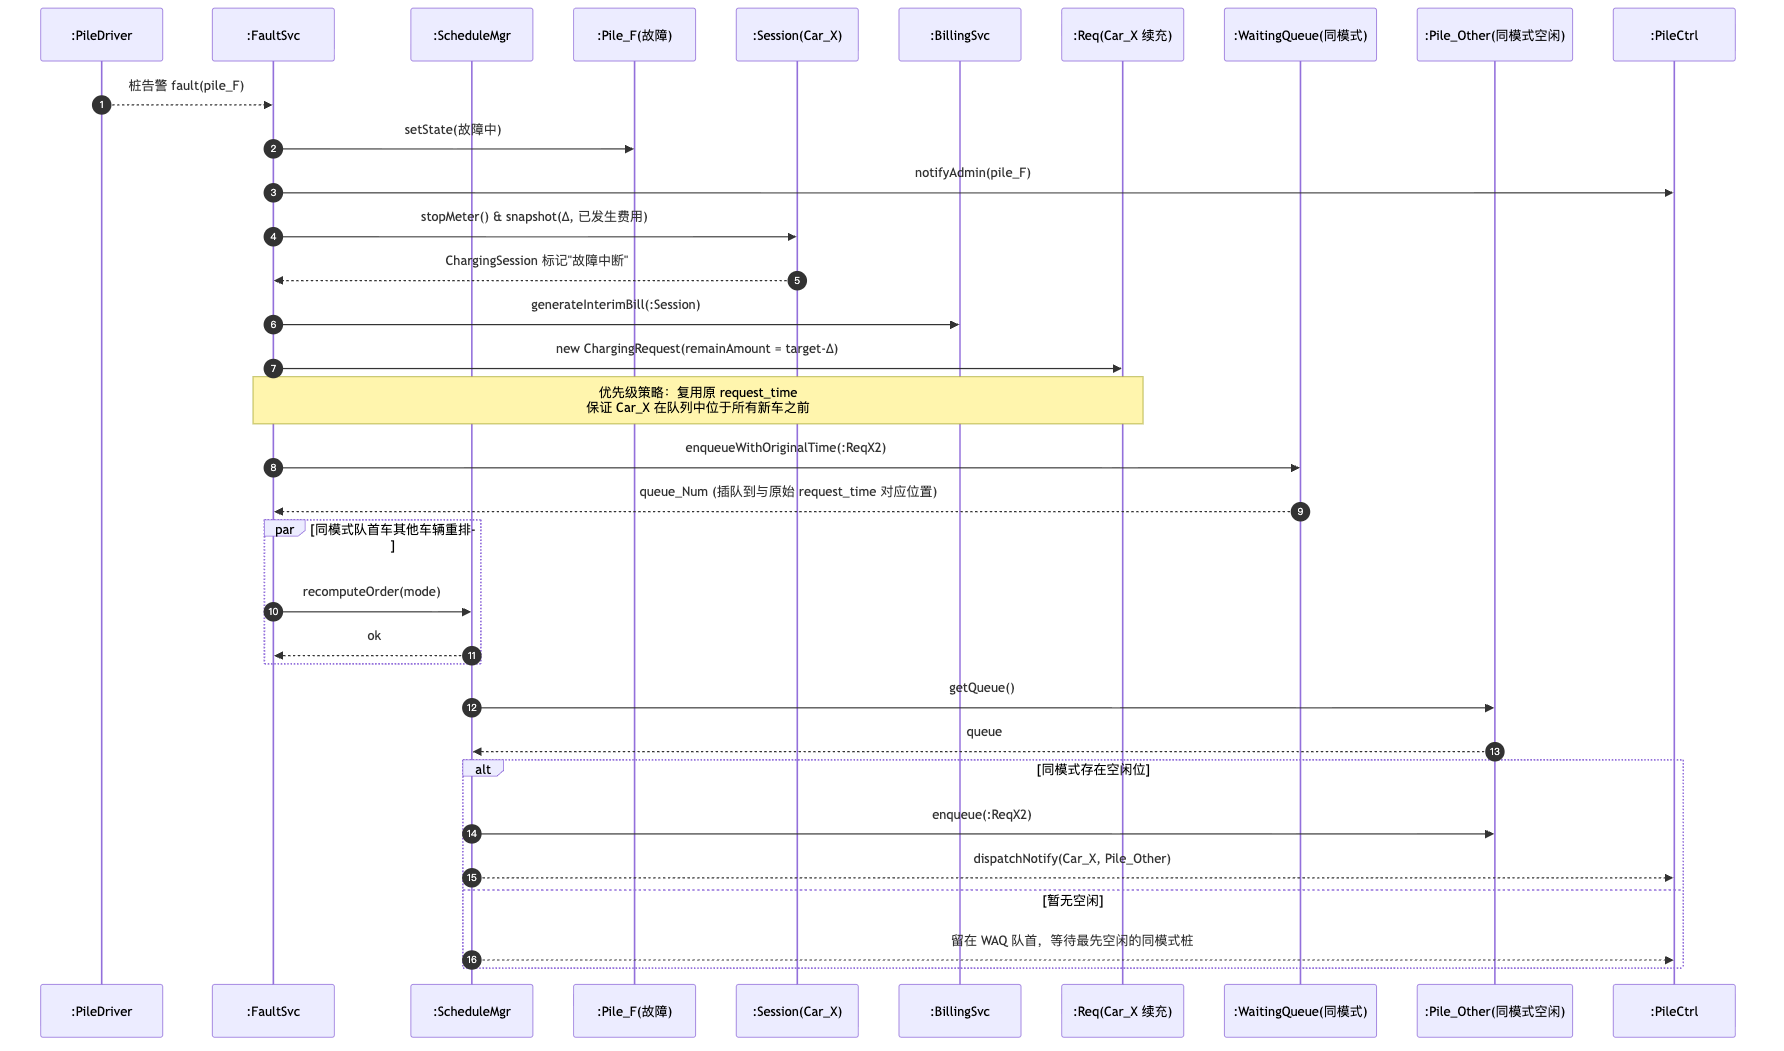
\includegraphics[width=0.97\linewidth]{diagram_17.png}
\end{figure}

\subsubsection{对象设计：时间顺序调度}

\textbf{问题与解决方案}

\begin{tabularx}{\linewidth}{p{5.4cm}Y}
\toprule
\textbf{问题} & \textbf{解决方案} \\
\midrule
受影响请求如何统一处理？ & 都退回到等待队列，按各自原 \texttt{request\_time} 重排，不区分``原本排队''和``被故障撞回来''。 \\
谁负责把桩内队列回流？ & \texttt{:FaultSvc.drainAllPendingTo(WAQ)} 把 \texttt{Pile\_F} 未开始的请求逐条 \texttt{enqueueByRequestTime}。 \\
\bottomrule
\end{tabularx}

\textbf{Sequence Diagram}

\begin{figure}[ht]
\centering
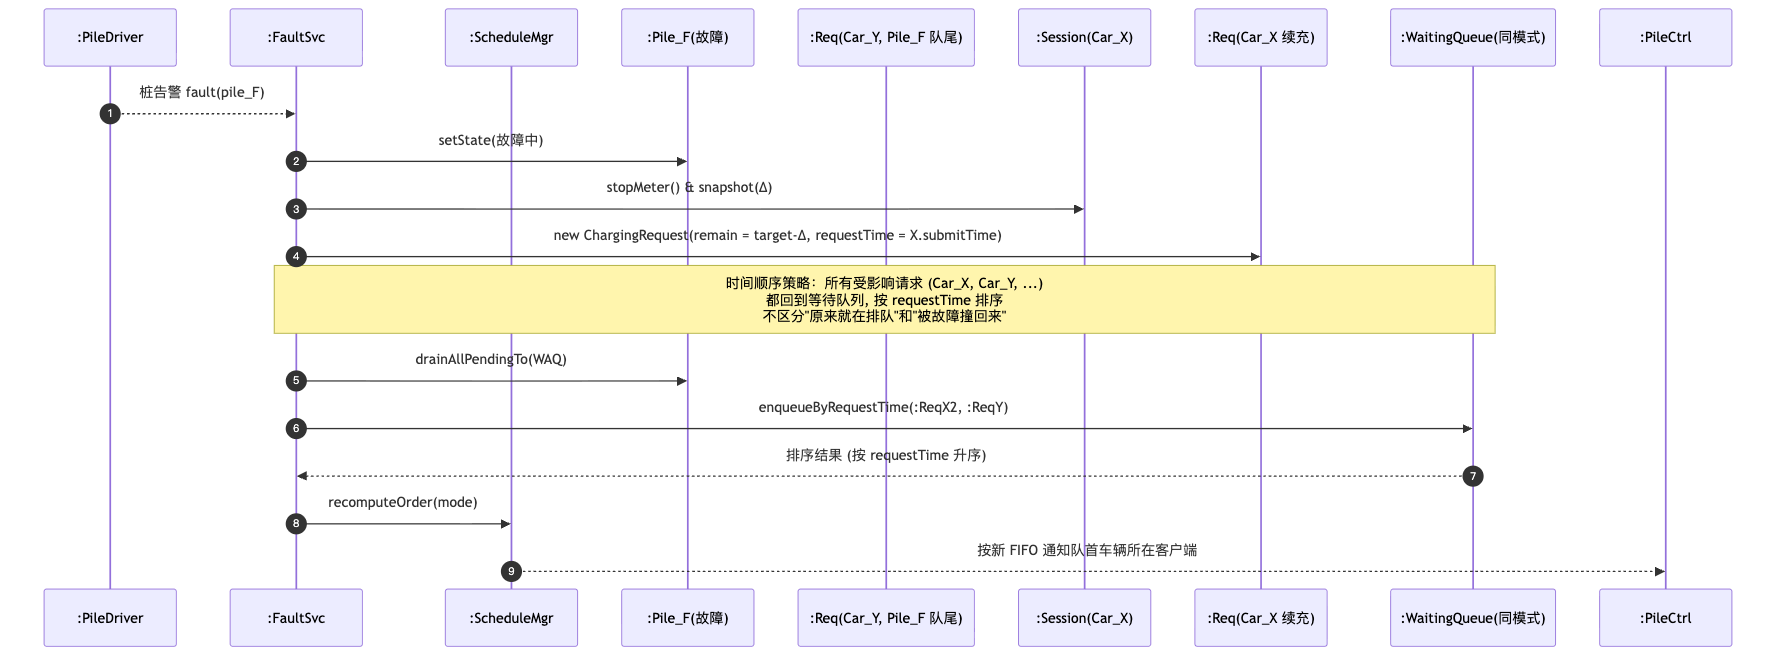
\includegraphics[width=0.97\linewidth]{diagram_18.png}
\end{figure}

\subsubsection{对象设计：充电中故障恢复}

\textbf{问题与解决方案}

\begin{tabularx}{\linewidth}{p{5.4cm}Y}
\toprule
\textbf{问题} & \textbf{解决方案} \\
\midrule
桩恢复后是否需要重启服务？ & 需要。\texttt{:PileSvc.resume} 先调 \texttt{:PileDriver.selfTest}，自检通过才 \texttt{setState(空闲)} 并 \texttt{registerAvailable}。 \\
``故障中断''会话费用如何与新账单合并？ & \texttt{:BillingSvc.finalizeInterruptedSessions(pile\_F)} 把快照费用合并到当前主账单（如有）。 \\
\bottomrule
\end{tabularx}

\textbf{Sequence Diagram}

\begin{figure}[ht]
\centering
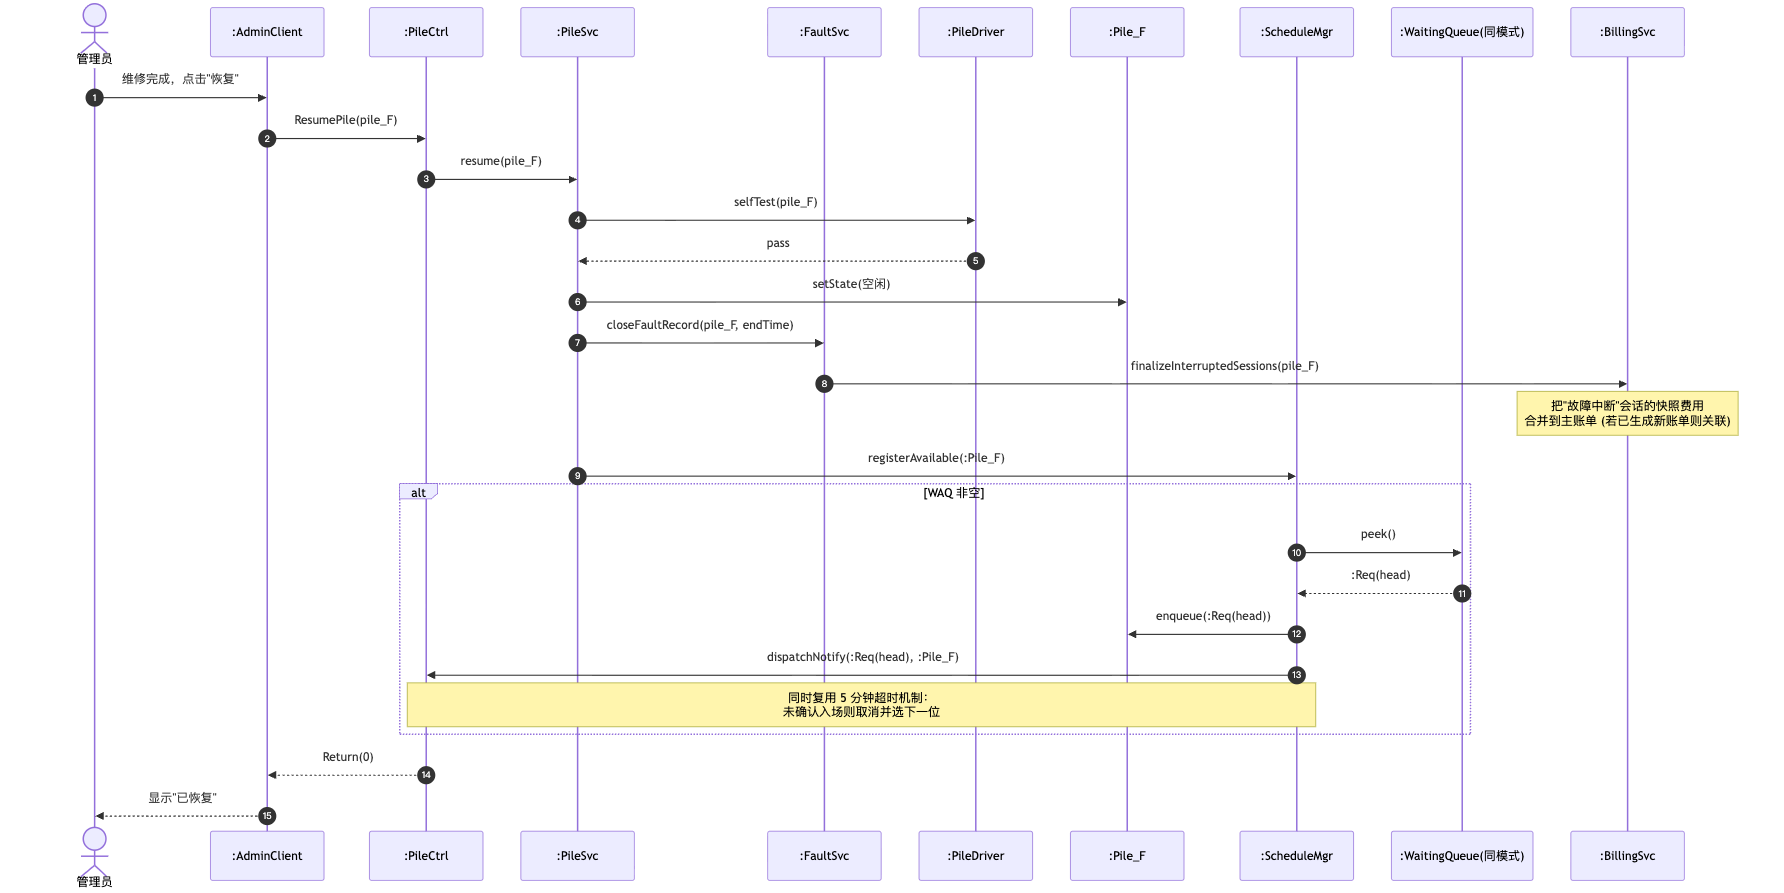
\includegraphics[width=0.97\linewidth]{diagram_19.png}
\end{figure}

\clearpage
%==========================================================
\subsection{可选加分调度策略}

本节面向作业要求中的两项可选加分项：单次调度总充电时长最短、批量调度总充电时长最短。两项都以``完成充电所需时间 = 等待时长 + 自己充电时长''为最小化目标，与 2.6 节互补：2.6 解决``出故障后受影响请求如何处理''，本节解决``当前请求进入充电区瞬间选哪个桩最优''。

形式化定义：设当前模式空闲桩集合为 \texttt{P*}，对每个候选 \texttt{p $\in$ P*}，候选请求 \texttt{r} 选择 \texttt{p} 的总完成时间为
$$T(r,p) = \mathrm{sum}(\mathrm{remain\_charge\_time\ of\ p's\ current\ queue}) + r.\mathrm{amount} / p.\mathrm{rate}.$$

\subsubsection{对象设计：单次调度总充电时长最短}

\textbf{问题与解决方案}

\begin{tabularx}{\linewidth}{p{5.4cm}Y}
\toprule
\textbf{问题} & \textbf{解决方案} \\
\midrule
决策粒度？ & 单次：每出队一辆车，独立选择当时使其 \texttt{T(r,p)} 最小的桩。 \\
其它车辆是否重排？ & 不重排，保持简单与可解释性。 \\
\bottomrule
\end{tabularx}

\textbf{Sequence Diagram}

\begin{figure}[ht]
\centering
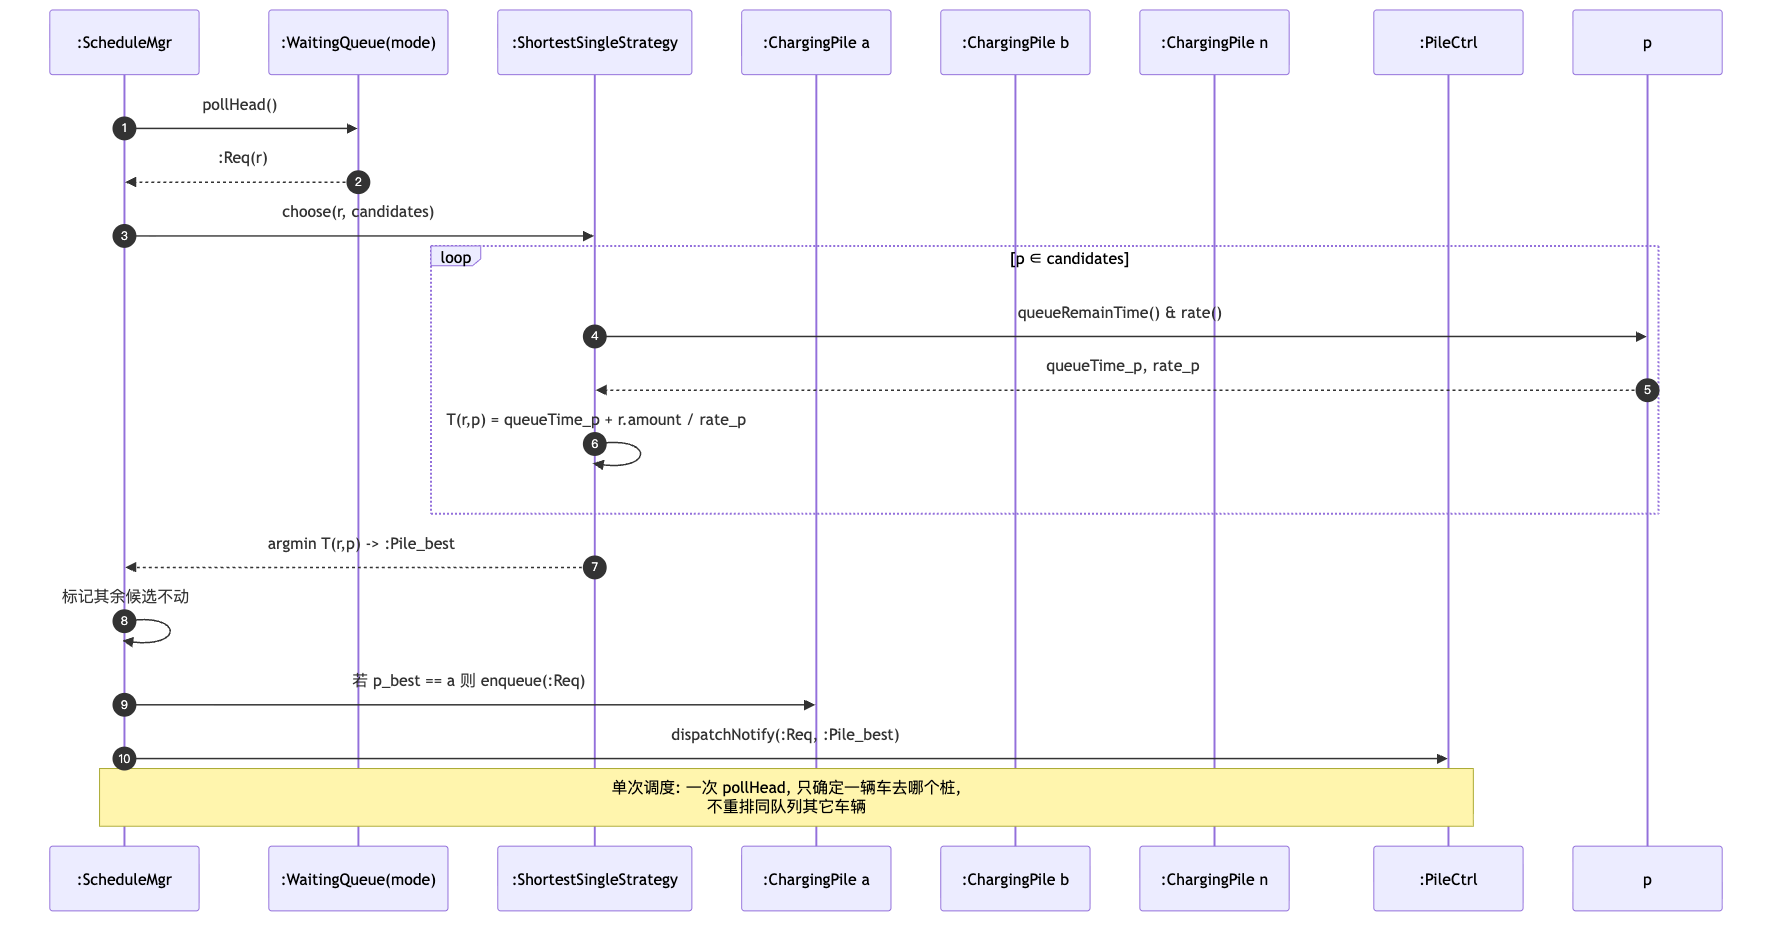
\includegraphics[width=0.95\linewidth]{diagram_20.png}
\end{figure}

\subsubsection{对象设计：批量调度总充电时长最短}

\textbf{问题与解决方案}

\begin{tabularx}{\linewidth}{p{5.4cm}Y}
\toprule
\textbf{问题} & \textbf{解决方案} \\
\midrule
何时触发批量优化？ & 周期性（例如调度 tick）或某桩进入空闲时一次性优化全部等待请求。 \\
是否破坏 FIFO？ & 在 FIFO 顺序内贪心选择最低 \texttt{ΔT} 的桩，保留先到先服务的相对顺序约束。 \\
\bottomrule
\end{tabularx}

\textbf{Sequence Diagram}

\begin{figure}[ht]
\centering
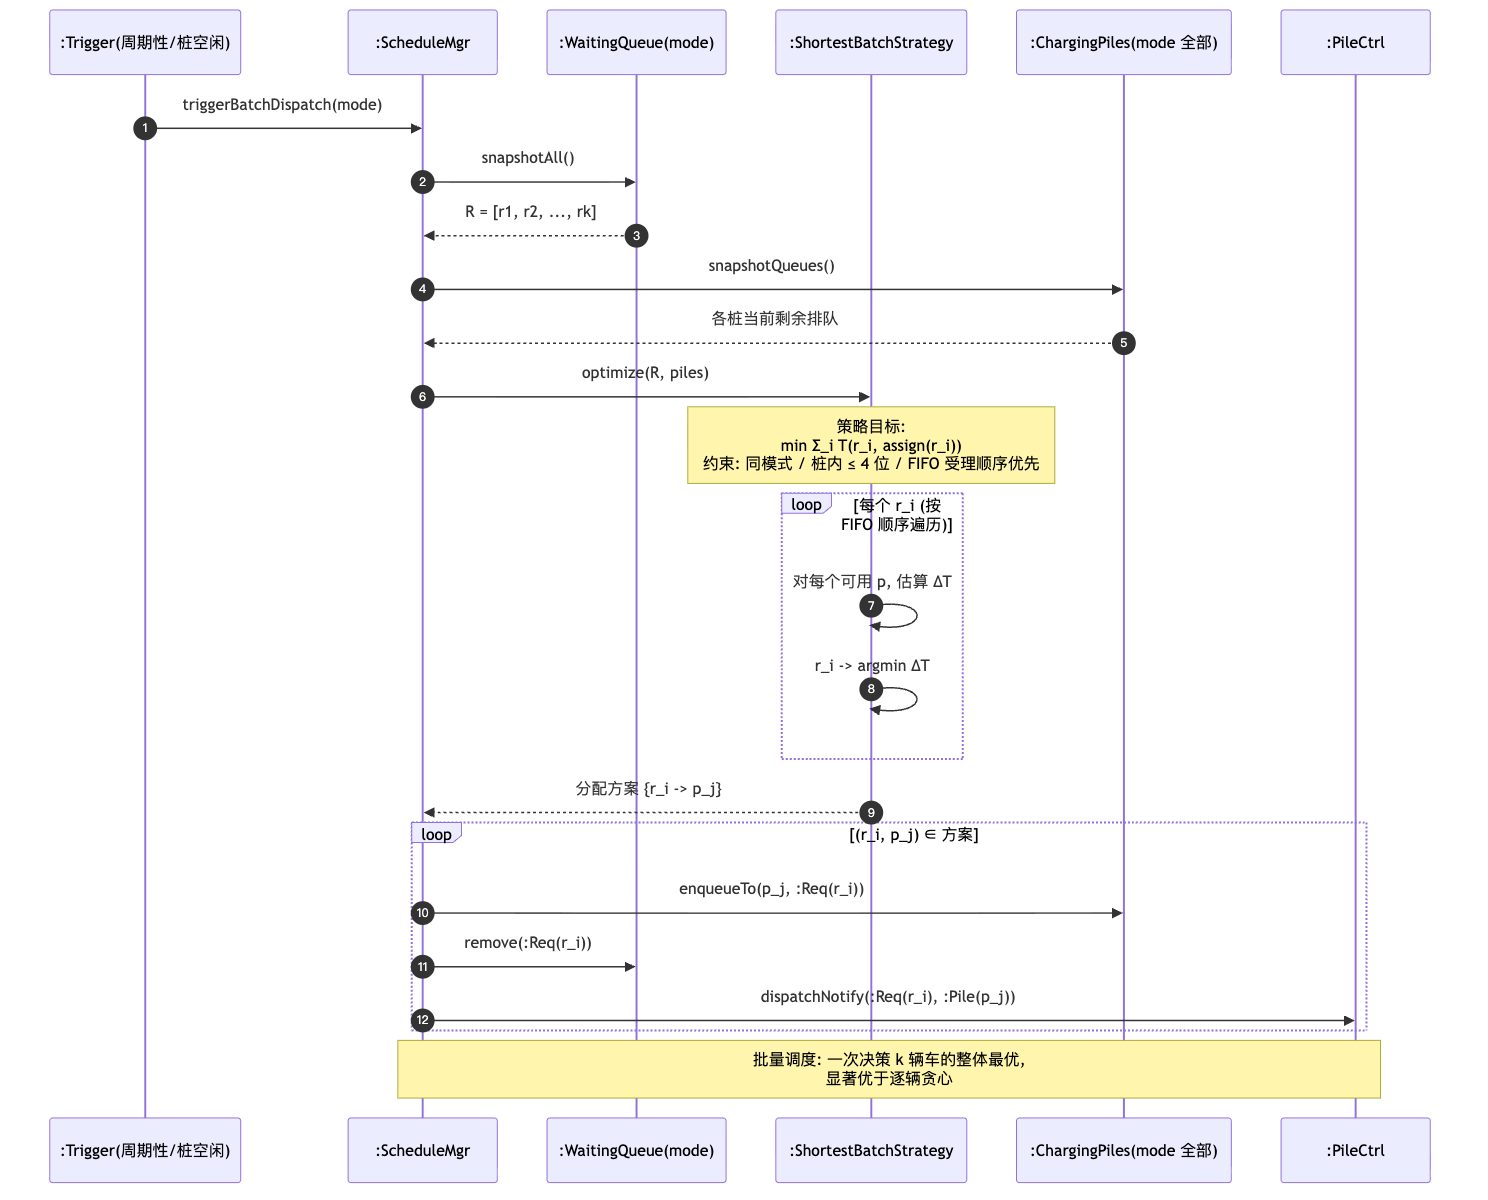
\includegraphics[width=0.97\linewidth]{diagram_21.png}
\end{figure}

\clearpage
%==========================================================
\section{静态结构设计 (10\%)}

本章按模版要求逐个用例给出``软件分层类图 + 类属性与方法说明表''，统一只使用依赖、定向关联、继承三种关系：

\begin{itemize}
\item \textbf{继承（Generalization）}：\texttt{$\triangleright$}，仅用于充电桩家族。
\item \textbf{定向关联（Directed Association）}：\texttt{$\longrightarrow$}，表示一个类持有另一个类的引用。
\item \textbf{依赖（Dependency）}：$\dashv\!\!\!\!\rightarrow$（虚线箭头），表示一个类在方法签名/调用中使用另一个类，但不持有其引用。
\end{itemize}

每张类图只包含本用例时序图涉及的类；继承自父类的成员不在子类表中重复列出。

\subsection{用例：充电申请}

\subsubsection{软件分层类图}

\begin{figure}[ht]
\centering
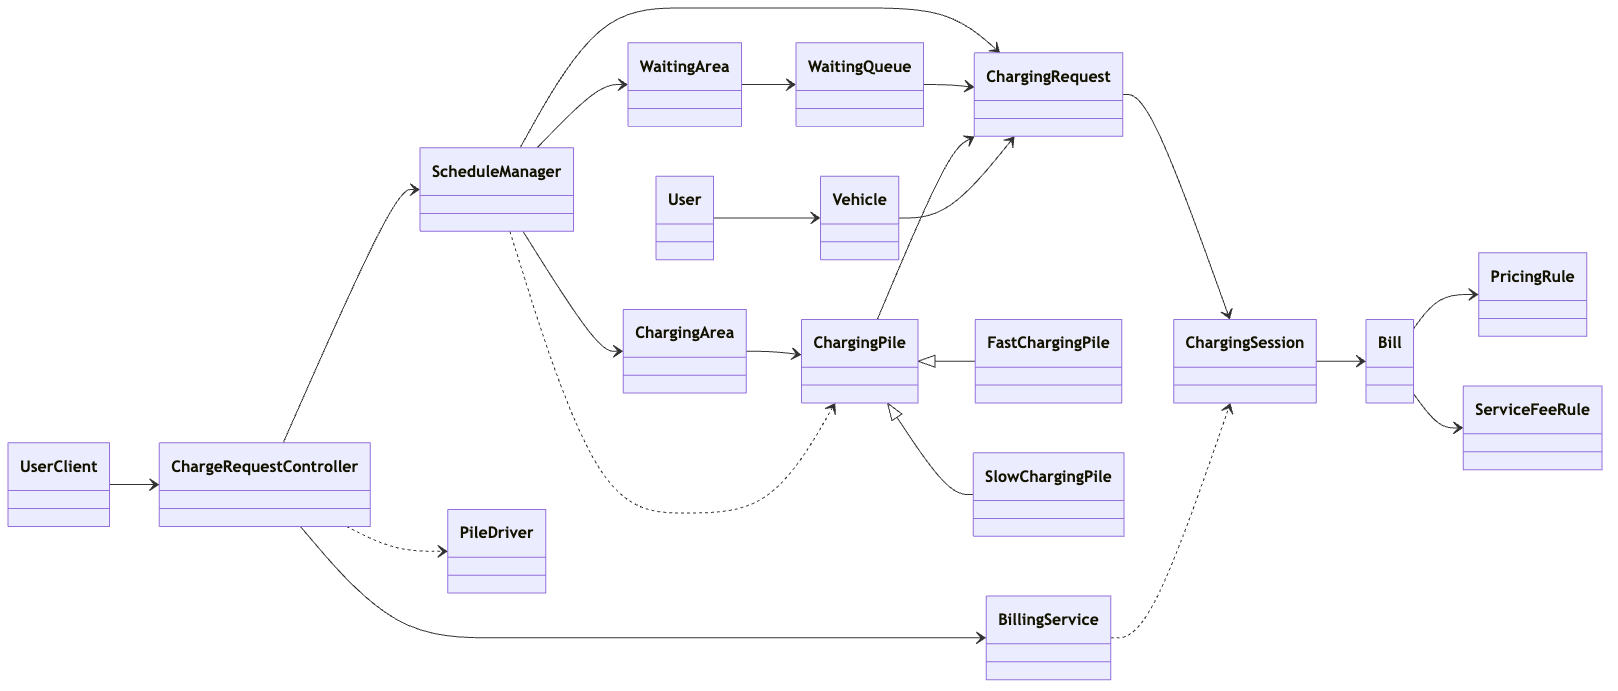
\includegraphics[width=0.97\linewidth]{diagram_22.png}
\end{figure}

\subsubsection{属性与方法说明}

\begin{longtable}{p{3.6cm}p{5.4cm}p{6.5cm}}
\toprule
\textbf{类名} & \textbf{主要属性} & \textbf{主要方法（与本用例消息对应）} \\
\midrule
\endhead
\texttt{UserClient} & currentUserId, currentVehicleId, sessionToken & submitChargeRequest(), modifyAmount(), modifyMode(), queryCarState(), startCharging(), queryChargingState(), endCharging() \\
\texttt{ChargeRequestController} & — & \texttt{E\_chargingRequest}, \texttt{Modify\_Amount}, \texttt{Modify\_Mode}, \texttt{Query\_Car\_State}, \texttt{Start\_Charging}, \texttt{Query\_Charging\_State}, \texttt{End\_Charging} \\
\texttt{ScheduleManager} & strategy, waitingArea, chargingArea & createRequest(), recomputeWaitTime(), validateOnPile(), onPileFreed() \\
\texttt{BillingService} & pricingRule, serviceRule & generateBill(), aggregateBills(), explodeDetail() \\
\texttt{WaitingArea} & capacity & getQueue(mode) \\
\texttt{WaitingQueue} & mode, items: List\textless ChargingRequest\textgreater & enqueue(), pollHead(), peek(), positionOf(), list(), remove() \\
\texttt{ChargingArea} & spotPerPile=4 & listPiles(), countFreeSpots() \\
\texttt{ChargingPile} & pileId, type, state, rate, totalChargeNum, totalChargeTime, totalCapacity, queue & getState(), setState(), enqueue(), peekHead(), queueRemainTime(), hasActiveSession() \\
\texttt{FastChargingPile} & rate=30kW & 继承自 \texttt{ChargingPile} \\
\texttt{SlowChargingPile} & rate=7kW & 继承自 \texttt{ChargingPile} \\
\texttt{ChargingRequest} & requestId, carId, mode, targetAmount, state, requestTime, queueNum, originalRequestTime & setState(), setTargetAmount(), getState(), getQueueNum(), getRequestTime() \\
\texttt{ChargingSession} & sessionId, requestId, pileId, startTime, endTime, kWh, duration, status & updateRealtime(), finalize(), stopMeter() \\
\texttt{Bill} & billId, sessionId, chargeAmount, chargeDuration, startTime, endTime, totalChargeFee, totalServiceFee, totalFee, payState & computeFromSession(), getDetail(), markPaid() \\
\texttt{PricingRule} & peakRate, normalRate, valleyRate, peakRange, valleyRange, validFrom & rateAt(time), ratesBetween(t1,t2) \\
\texttt{ServiceFeeRule} & rate, validFrom & rate() \\
\texttt{PileDriver} & endpoints: Map\textless pileId, ConnectionInfo\textgreater & startCharging(), stopCharging(), pullRealtime() \\
\texttt{User} & userId, userName & hasOverdueBill(), addVehicle() \\
\texttt{Vehicle} & vehicleId, carCapacity & getOwner(), getActiveRequest() \\
\bottomrule
\end{longtable}

\clearpage
\subsection{用例：查看账单 / 查看详单}

\subsubsection{软件分层类图}

\begin{figure}[ht]
\centering
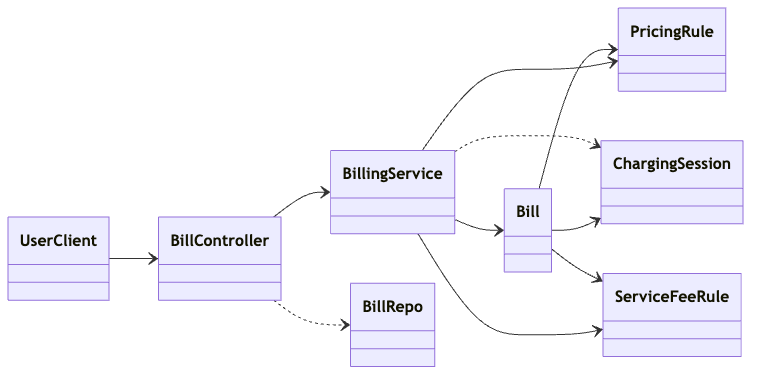
\includegraphics[width=0.92\linewidth]{diagram_23.png}
\end{figure}

\subsubsection{属性与方法说明}

\begin{longtable}{p{3.4cm}p{5.6cm}p{6.5cm}}
\toprule
\textbf{类名} & \textbf{主要属性} & \textbf{主要方法} \\
\midrule
\endhead
\texttt{UserClient} & currentUserId & requestBill(), requestDetailedList() \\
\texttt{BillController} & — & \texttt{Request\_Bill}, \texttt{Request\_DetailedList} \\
\texttt{BillingService} & pricingRule, serviceRule & aggregateBills(), explodeDetail() \\
\texttt{Bill} & billId, sessionId, carId, date, chargeAmount, chargeDuration, startTime, endTime, totalChargeFee, totalServiceFee, totalFee & getSession(), getDetail() \\
\texttt{ChargingSession} & sessionId, pileId, startTime, endTime, kWh & finalize() \\
\texttt{PricingRule} & peakRate, normalRate, valleyRate, peakRange, valleyRange & rateAt(time), ratesBetween(t1,t2) \\
\texttt{ServiceFeeRule} & rate & rate() \\
\texttt{BillRepo} & — & findByCarAndDate(), findById() \\
\bottomrule
\end{longtable}

\clearpage
\subsection{用例：运行充电桩}

\subsubsection{软件分层类图}

\begin{figure}[ht]
\centering
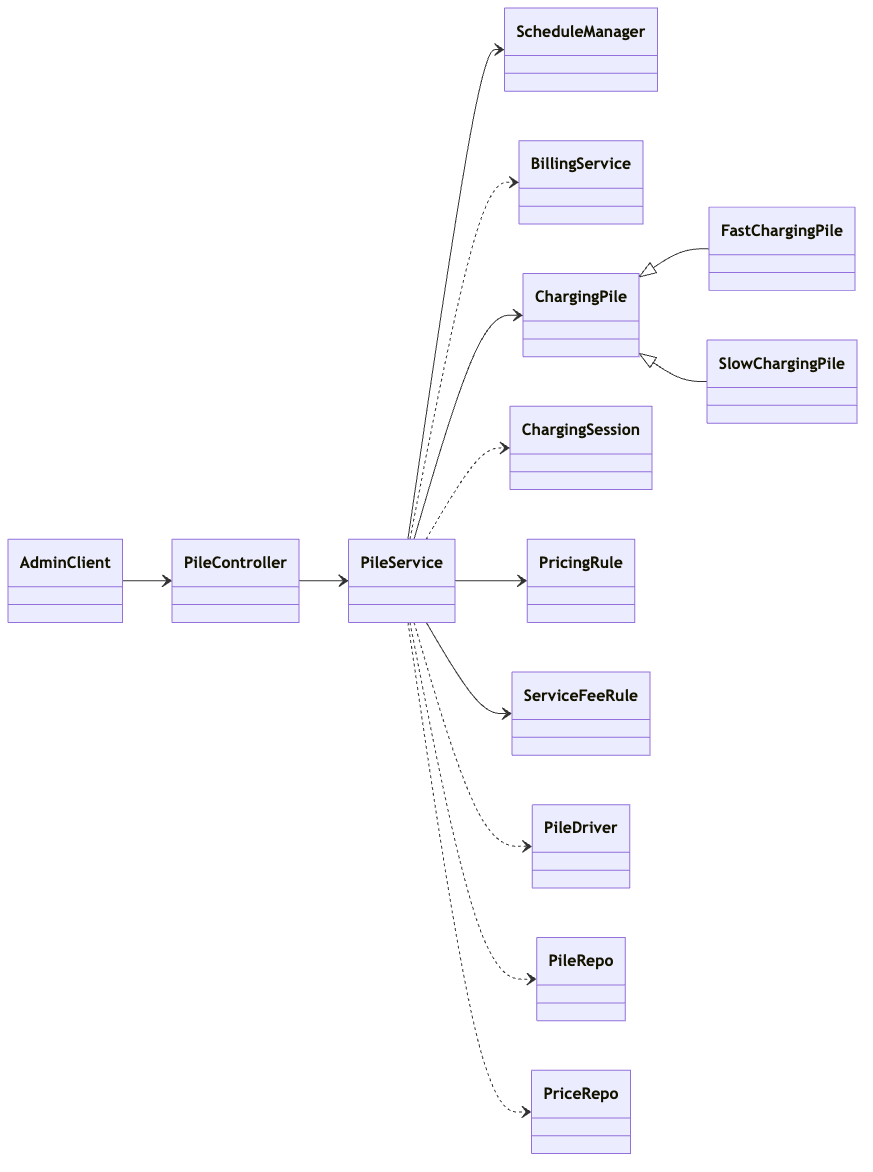
\includegraphics[width=0.97\linewidth]{diagram_24.png}
\end{figure}

\subsubsection{属性与方法说明}

\begin{longtable}{p{3.4cm}p{5.6cm}p{6.5cm}}
\toprule
\textbf{类名} & \textbf{主要属性} & \textbf{主要方法} \\
\midrule
\endhead
\texttt{AdminClient} & adminId & powerOn(), setParameters(), startChargingPile(), powerOff() \\
\texttt{PileController} & — & \texttt{powerOn}, \texttt{setParameters}, \texttt{Start\_ChargingPile}, \texttt{powerOff} \\
\texttt{PileService} & — & powerOn(), powerOff(), start(), applyParameters() \\
\texttt{ScheduleManager} & strategy & registerAvailable(), unregisterAvailable(), returnWaitersToWaitingArea() \\
\texttt{BillingService} & pricingRule, serviceRule & generateBill() \\
\texttt{ChargingPile} & pileId, type, state, rate, totalChargeNum, totalChargeTime, totalCapacity & getState(), setState(), hasActiveSession() \\
\texttt{FastChargingPile} & rate=30kW & 继承 \\
\texttt{SlowChargingPile} & rate=7kW & 继承 \\
\texttt{ChargingSession} & sessionId, kWh, duration & finalize(), snapshot() \\
\texttt{PricingRule} & peakRate, normalRate, valleyRate, validFrom & update() \\
\texttt{ServiceFeeRule} & rate, validFrom & update() \\
\texttt{PileDriver} & endpoints & powerOn(), powerOff(), startService(), stopService(), pushParam() \\
\texttt{PileRepo} & — & save(), snapshot() \\
\texttt{PriceRepo} & — & save() \\
\bottomrule
\end{longtable}

\clearpage
\subsection{用例：查看充电桩状态 / 查看队列状态}

\subsubsection{软件分层类图}

\begin{figure}[ht]
\centering
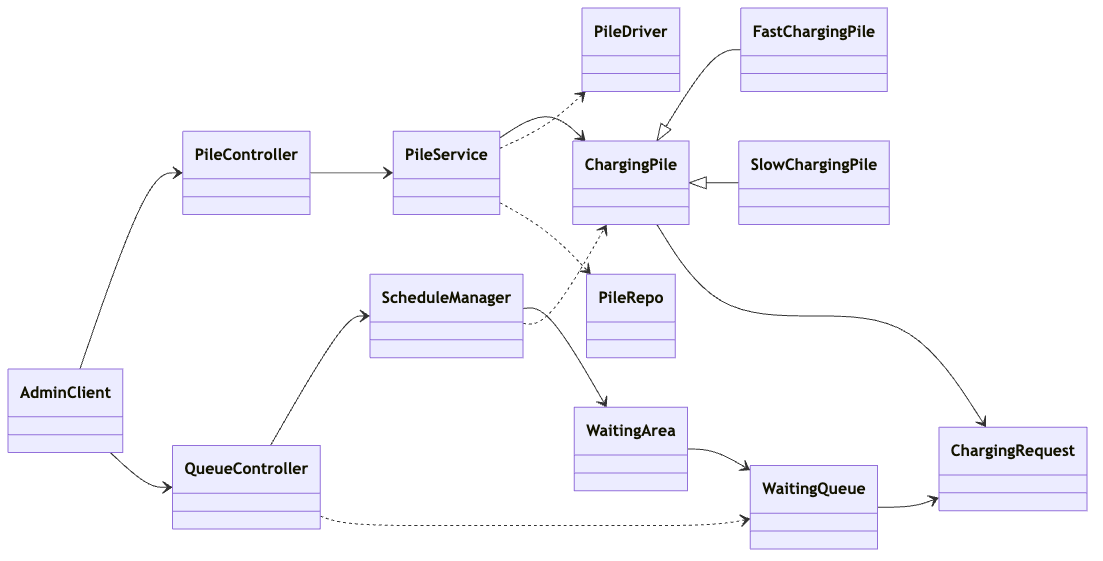
\includegraphics[width=0.97\linewidth]{diagram_25.png}
\end{figure}

\subsubsection{属性与方法说明}

\begin{longtable}{p{3.6cm}p{5.4cm}p{6.5cm}}
\toprule
\textbf{类名} & \textbf{主要属性} & \textbf{主要方法} \\
\midrule
\endhead
\texttt{AdminClient} & adminId, refreshInterval & queryPileState(), queryQueueState() \\
\texttt{PileController} & — & \texttt{Query\_PileState} \\
\texttt{QueueController} & — & \texttt{Query\_QueueState} \\
\texttt{PileService} & — & queryState() \\
\texttt{ScheduleManager} & — & snapshot(queueId), estimateWaitTime() \\
\texttt{ChargingPile} & pileId, workingState, totalChargeNum, totalChargeTime, totalCapacity, queue & getWorkingState(), getQueue(), queueRemainTime(), pullCounters() \\
\texttt{FastChargingPile}, \texttt{SlowChargingPile} & rate=30/7kW & 继承 \\
\texttt{WaitingArea} & — & getQueue(mode) \\
\texttt{WaitingQueue} & mode, items & list(), positionOf() \\
\texttt{ChargingRequest} & requestId, carId, carCapacity, requestAmount, requestTime & getState() \\
\texttt{PileDriver} & endpoints & pullCounters() \\
\texttt{PileRepo} & — & snapshot() \\
\bottomrule
\end{longtable}

\clearpage
\subsection{用例：调度对象核心交互}

\subsubsection{软件分层类图}

\begin{figure}[ht]
\centering
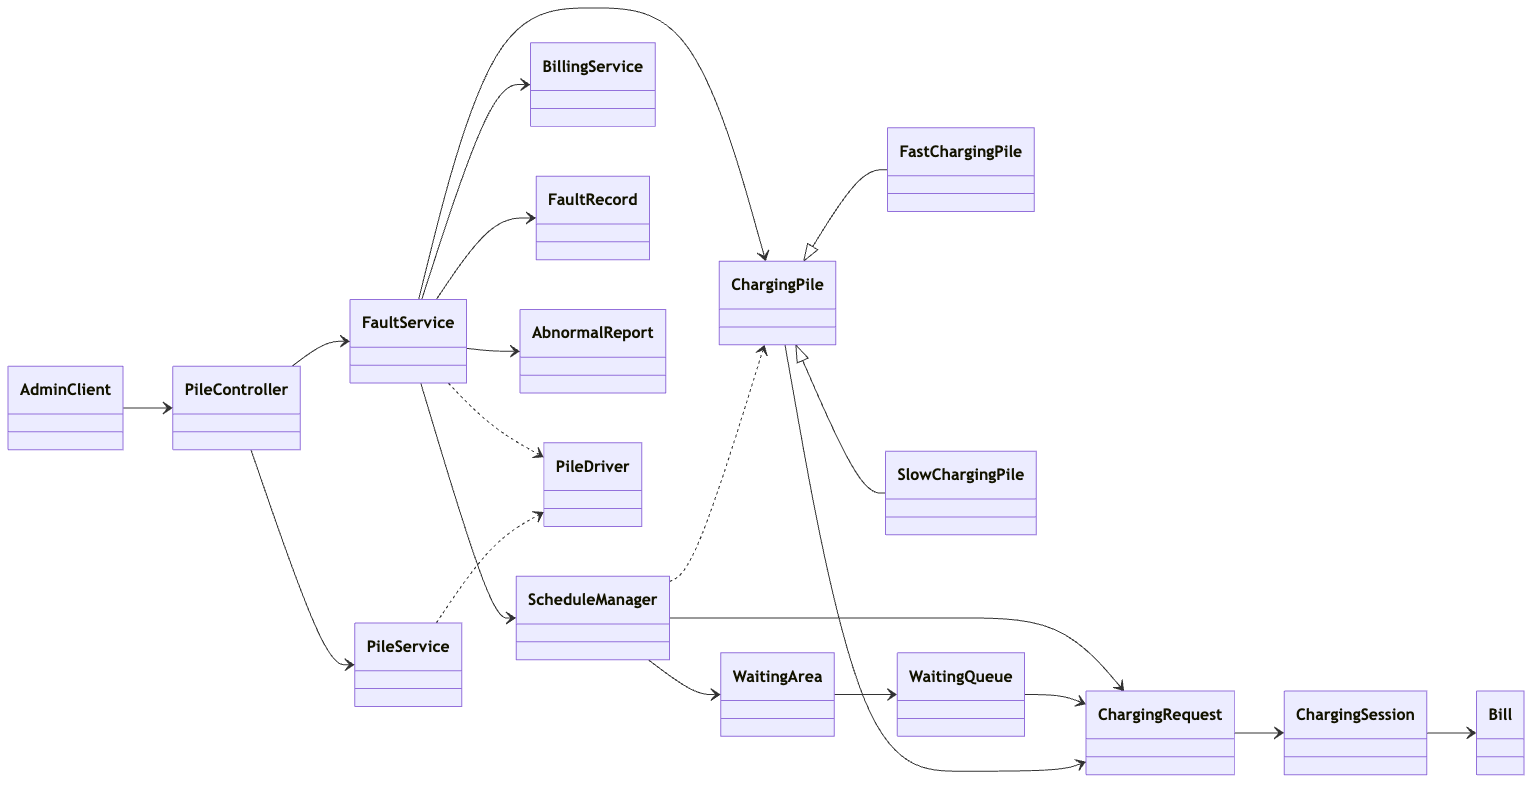
\includegraphics[width=0.97\linewidth]{diagram_26.png}
\end{figure}

\subsubsection{属性与方法说明}

\begin{longtable}{p{3.6cm}p{5.4cm}p{6.5cm}}
\toprule
\textbf{类名} & \textbf{主要属性} & \textbf{主要方法} \\
\midrule
\endhead
\texttt{AdminClient} & adminId & confirmPileFault(), resumePile() \\
\texttt{PileController} & — & \texttt{ConfirmPileFault}, \texttt{ResumePile}, \texttt{notifyAdmin} \\
\texttt{PileService} & — & resume() \\
\texttt{FaultService} & activeFaults: Map\textless pileId, FaultRecord\textgreater & onPileFault(), drainAllPendingTo(), closeFaultRecord(), recomputeOrderAfterFault(), finalizeInterruptedSessions() \\
\texttt{ScheduleManager} & strategy & recomputeOrder(mode), registerAvailable(), dispatchNotify() \\
\texttt{BillingService} & pricingRule, serviceRule & generateInterimBill(), finalizeInterruptedSessions() \\
\texttt{ChargingPile} & pileId, state, queue, rate & setState(), getQueue(), drainAllPendingTo() \\
\texttt{FastChargingPile}, \texttt{SlowChargingPile} & rate & 继承 \\
\texttt{WaitingArea} / \texttt{WaitingQueue} & — & enqueueWithOriginalTime(), enqueueByRequestTime(), peek() \\
\texttt{ChargingRequest} & requestId, carId, mode, targetAmount, state, requestTime, originalRequestTime & setState() \\
\texttt{ChargingSession} & sessionId, kWh, status, snapshotFee & stopMeter(), snapshot() \\
\texttt{Bill} & billId, sessionId, totalFee, payState & computeFromSession() \\
\texttt{FaultRecord} & faultId, pileId, faultType, faultTime, endTime, sourceReportId & open(), close() \\
\texttt{AbnormalReport} & reportId, userId, pileId, description, reportTime & bindTo(pile) \\
\texttt{PileDriver} & endpoints & selfTest() \\
\bottomrule
\end{longtable}

\clearpage
\subsection{系统级的静态结构（可选）}

把上述五个用例的类与关系合并，得到本系统的总体软件分层结构。仍然只使用模版要求的三种关系。

\begin{figure}[ht]
\centering
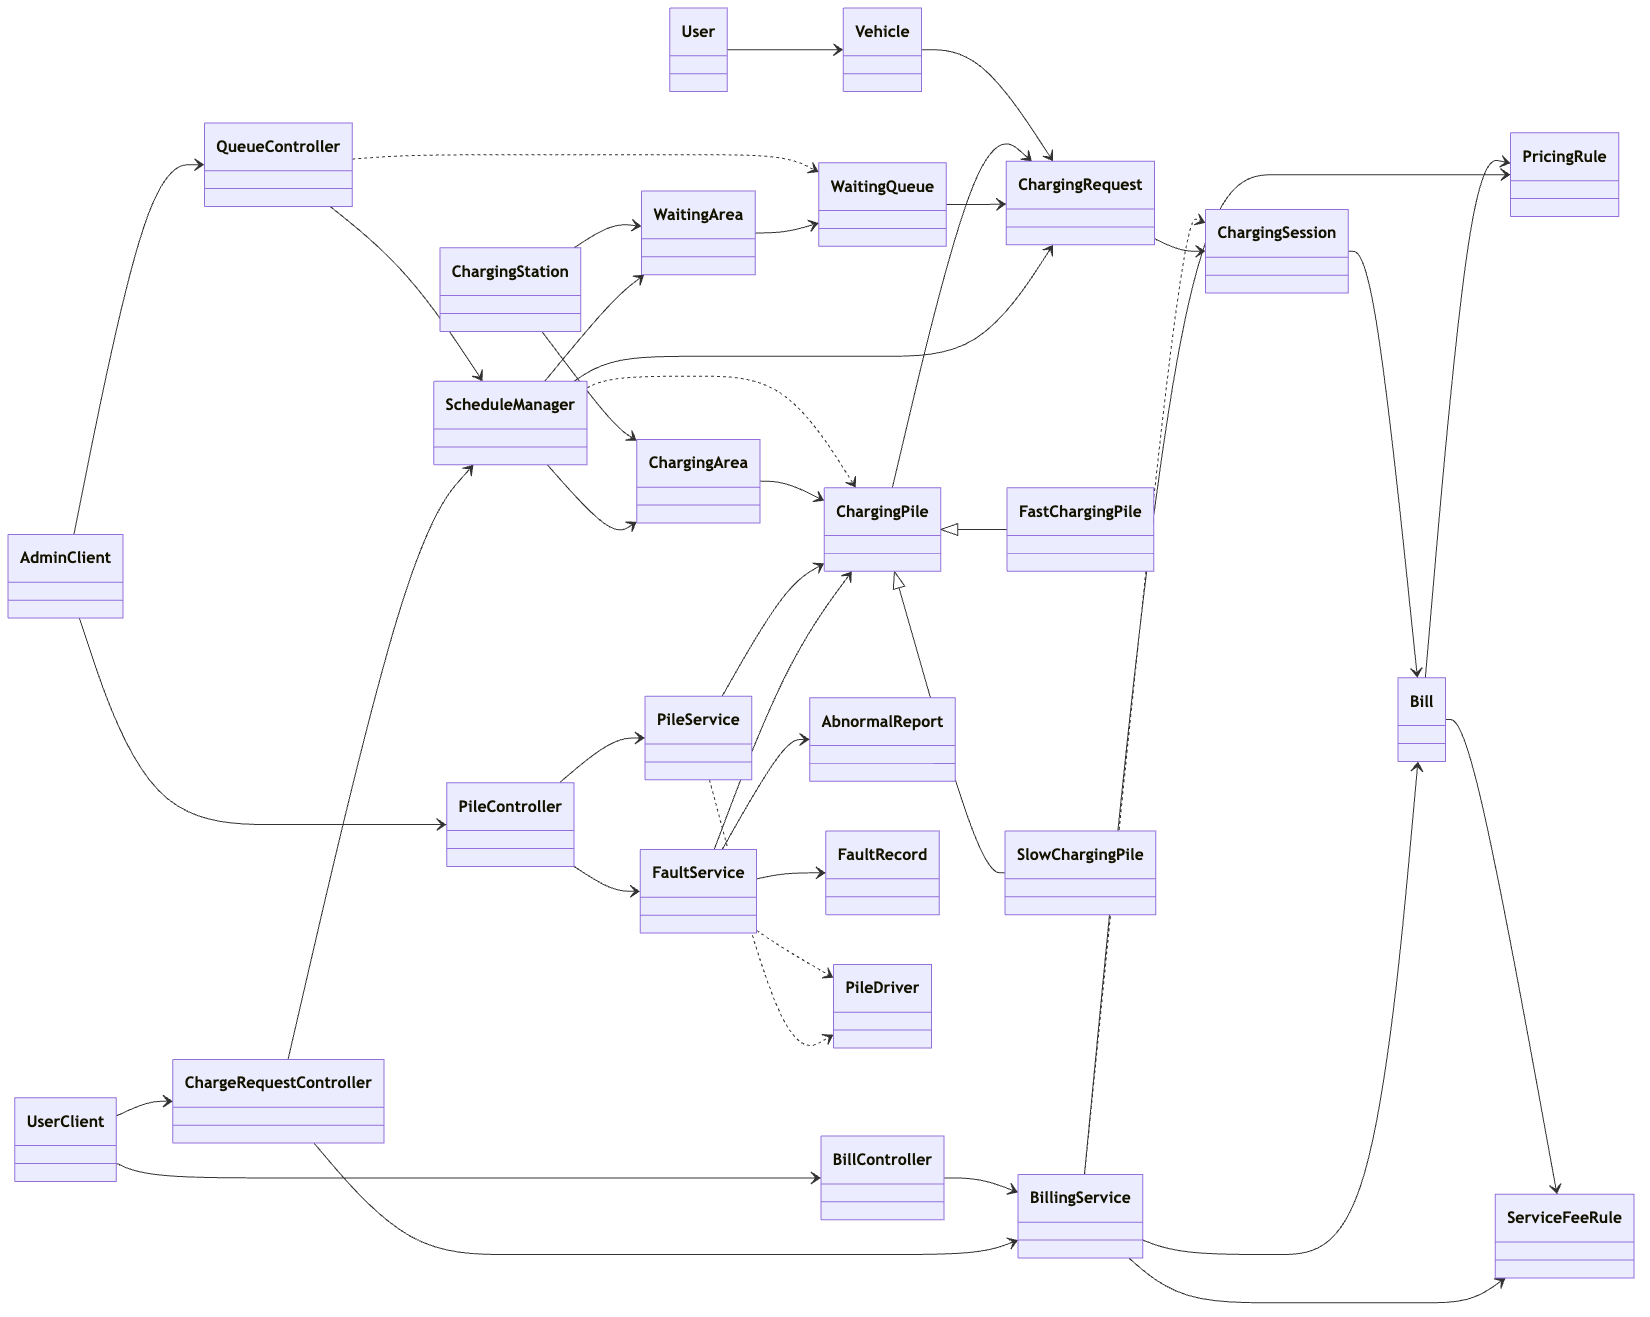
\includegraphics[width=0.99\linewidth]{diagram_27.png}
\end{figure}

\noindent 图中刻意避免使用聚合 / 组合 / 关联类等 HW1 已使用过的关系符号；本次只保留作业要求的三种关系，所有``整体-局部''语义统一弱化为``定向关联''。各类的属性与方法详见 3.1$\sim$3.5 节按用例给出的说明表。

\clearpage
%==========================================================
\section{系统事件人员分配}

本节按作业要求给出``系统事件 → 责任人''的分工，便于评审追踪。为落实``一个任务尽量由一人独立完成''的要求，下表中每个系统事件均只指定唯一负责人，由其独立完成该事件的时序图与设计。其中调度交互与加分项属核心难点，由组长唐振桓负责；杨凌俊承担充电桩运行等较多事件，故唐振桓、杨凌俊二人任务量最多，其余事件分给袁炜途、马迪轩、刘宇轩。仅统稿、文档美化、交叉复核等整体性工作仍由全组协同（详见后表）。

\subsection{系统事件分工表}

\begin{longtable}{p{3.0cm}p{6.4cm}p{2.8cm}}
\toprule
\textbf{类别} & \textbf{系统事件} & \textbf{负责人} \\
\midrule
\endhead
充电申请 & \texttt{E\_chargingRequest} & 杨凌俊 \\
充电申请 & \texttt{Modify\_Amount} & 杨凌俊 \\
充电申请 & \texttt{Modify\_Mode} & 袁炜途 \\
充电申请 & \texttt{Query\_Car\_State} & 袁炜途 \\
充电申请 & \texttt{Start\_Charging} & 马迪轩 \\
充电申请 & \texttt{Query\_Charging\_State} & 马迪轩 \\
充电申请 & \texttt{End\_Charging} & 袁炜途 \\
查看账单 & \texttt{Request\_Bill} & 刘宇轩 \\
查看详单 & \texttt{Request\_DetailedList} & 刘宇轩 \\
运行充电桩 & \texttt{powerOn} & 杨凌俊 \\
运行充电桩 & \texttt{setParameters} & 马迪轩 \\
运行充电桩 & \texttt{Start\_ChargingPile} & 杨凌俊 \\
运行充电桩 & \texttt{powerOff} & 杨凌俊 \\
查看充电桩状态 & \texttt{Query\_PileState} & 刘宇轩 \\
查看队列状态 & \texttt{Query\_QueueState} & 袁炜途 \\
调度交互（组长） & 优先级调度 & \textbf{唐振桓} \\
调度交互（组长） & 时间顺序调度 & \textbf{唐振桓} \\
调度交互（组长） & 充电中故障恢复 & \textbf{唐振桓} \\
加分项 & 单次调度总充电时长最短 & \textbf{唐振桓} \\
加分项 & 批量调度总充电时长最短 & \textbf{唐振桓} \\
\bottomrule
\end{longtable}

\subsection{文档与统稿分工}

\begin{longtable}{p{4.6cm}ccccc}
\toprule
\textbf{工作项} & 唐振桓 & 杨凌俊 & 袁炜途 & 马迪轩 & 刘宇轩 \\
\midrule
\endhead
第一章 系统架构选择及说明 & √ & √ & & & \\
第二章 时序图绘制 & & √ & √ & √ & √ \\
第三章 用例级类图与说明表 & √ & √ & √ & & \\
调度对象交互（2.6 节） & √ & & & & \\
加分项策略（2.7 节） & √ & & & & \\
文档排版与目录 & & & & √ & √ \\
全文复核与提交 & & √ & √ & & \\
\bottomrule
\end{longtable}

\end{document}
